\documentclass[orivec]{llncs}
\usepackage{graphicx}
\usepackage{amsmath}			% for "cases"
\usepackage{amsfonts}		% for frakur fonts
\usepackage{mathrsfs}		% for curly "E" error symbol
\usepackage{float}
\usepackage{tcolorbox}		% for wrapping example in color box
\usepackage{wrapfig}			% wrap figure beside text, used in example
\usepackage{tikz-cd}			% commutative diagrams
\usepackage{tikz}
\usetikzlibrary{calc}
\usepackage{amssymb}			% for \multimap, \updownarrow, \bigstar
\usepackage{sectsty}			% change section color
% \usepackage{turnstile}		% longer turnstiles
\usepackage{wasysym}			% smileys
\usepackage[normalem]{ulem}	% underline with line breaks: /uline
% \usepackage{cancel}			% center "not" line for "broken heart"

\usepackage{geometry}		% change paper size
\geometry{
  a4paper,         % or letterpaper
  textwidth=18cm,  % llncs has 12.2cm
  textheight=27cm, % llncs has 19.3cm
  heightrounded,   % integer number of lines
  hratio=1:1,      % horizontally centered
  vratio=2:3,      % not vertically centered
}
\usepackage[fontsize=13pt]{scrextend}

% *************** Delete when not using Chinese or colors **********************
\usepackage{xeCJK}
\setCJKmainfont[BoldFont=SimHei,ItalicFont=KaiTi]{SimSun}
\usepackage{color}
\definecolor{Cerulean}{RGB}{100,100,200}
\newcommand{\emp}[1]{\textbf{\textcolor{Cerulean}{#1}}}
\definecolor{grey}{rgb}{0.9,0.9,0.9}  % grey

% \chapterfont{\color{blue}}  % sets colour of chapters
\sectionfont{\color{blue}} 
\subsectionfont{\color{blue}} 
\subsubsectionfont{\color{blue}} 

\newcommand{\vect}[1]{\boldsymbol{#1}}
\newcommand*\sigmoid{\vcenter{\hbox{
\includegraphics{sigmoid.png}}}}
\newcommand*\KB{\vcenter{\hbox{
\includegraphics{KB-symbol.png}}}}
\newcommand*\invsigmoid{\vcenter{\hbox{
\includegraphics{inverse-sigmoid.png}}}}
\newcommand{\invW}{\, \rotatebox[origin=c]{90}{W}}
\newcommand{\invw}{\, \rotatebox[origin=c]{90}{w}}
\newcommand*\rectifier{\vcenter{\hbox{
\includegraphics{rectifier.png}}}}
\newcommand{\dashh}{\textemdash~}

\newcommand{\tikzmark}[1]{\tikz[overlay,remember picture] \node (#1) {};}

%\makeatletter
%\@addtoreset{footnote}{page}
%\makeatother

%\renewcommand{\thefootnote}{\ensuremath{\ifcase\value{footnote}\or \dagger\or \dagger\dagger\or \ddagger\or \#\or \#\#\or \#\#\# \else\@ctrerr\fi}}

%\def\@fnsymbol#1{\ensuremath{\ifcase#1\or \dagger\or \ddagger\or \dagger\dagger \else\@ctrerr\fi}}
\renewcommand{\thefootnote}{\fnsymbol{footnote}}
\interfootnotelinepenalty=10000

% ***** Boxed variables inside math equations
% \newcommand*{\boxedcolor}{black}
\makeatletter
% \renewcommand{\boxed}[1]{\textcolor{\boxedcolor}{%
% \fbox{\normalcolor\m@th$\displaystyle#1$}}}
% \setlength{\fboxsep}{1pt}
\renewcommand{\boxed}[1]{\fbox{\m@th$\displaystyle\scalebox{0.9}{#1}$} \,}
\makeatother

\overfullrule=0mm

\newsavebox{\MyName}
\savebox{\MyName}{
\includegraphics[scale=0.6]{YKY.png}}

\title{记忆的结构}
\titlerunning{记忆的结构}
\author{\usebox{\MyName} (King-Yin Yan)
% \\ \footnotesize{General.Intelligence@Gmail.com}
}
\institute{General.Intelligence@Gmail.com}

\begin{document}

\maketitle
\setlength{\parindent}{0em}
% \setlength{\parskip}{2.8ex plus0.8ex minus0.8ex}
\setlength{\parskip}{2.8ex}

\begin{abstract}
(Draft...) 智能系统中记忆的设计似乎是一个比较 open-ended question。
\end{abstract}

\textbf{深度学习} 在近年很火,但 deep NN 的缺点是没有\textbf{记忆}。 有限自动机 (finite state machines) 不是\textbf{全能}的计算器,它和 Turing machine 的分别就是缺少了那条「记忆磁带」:
\begin{equation}
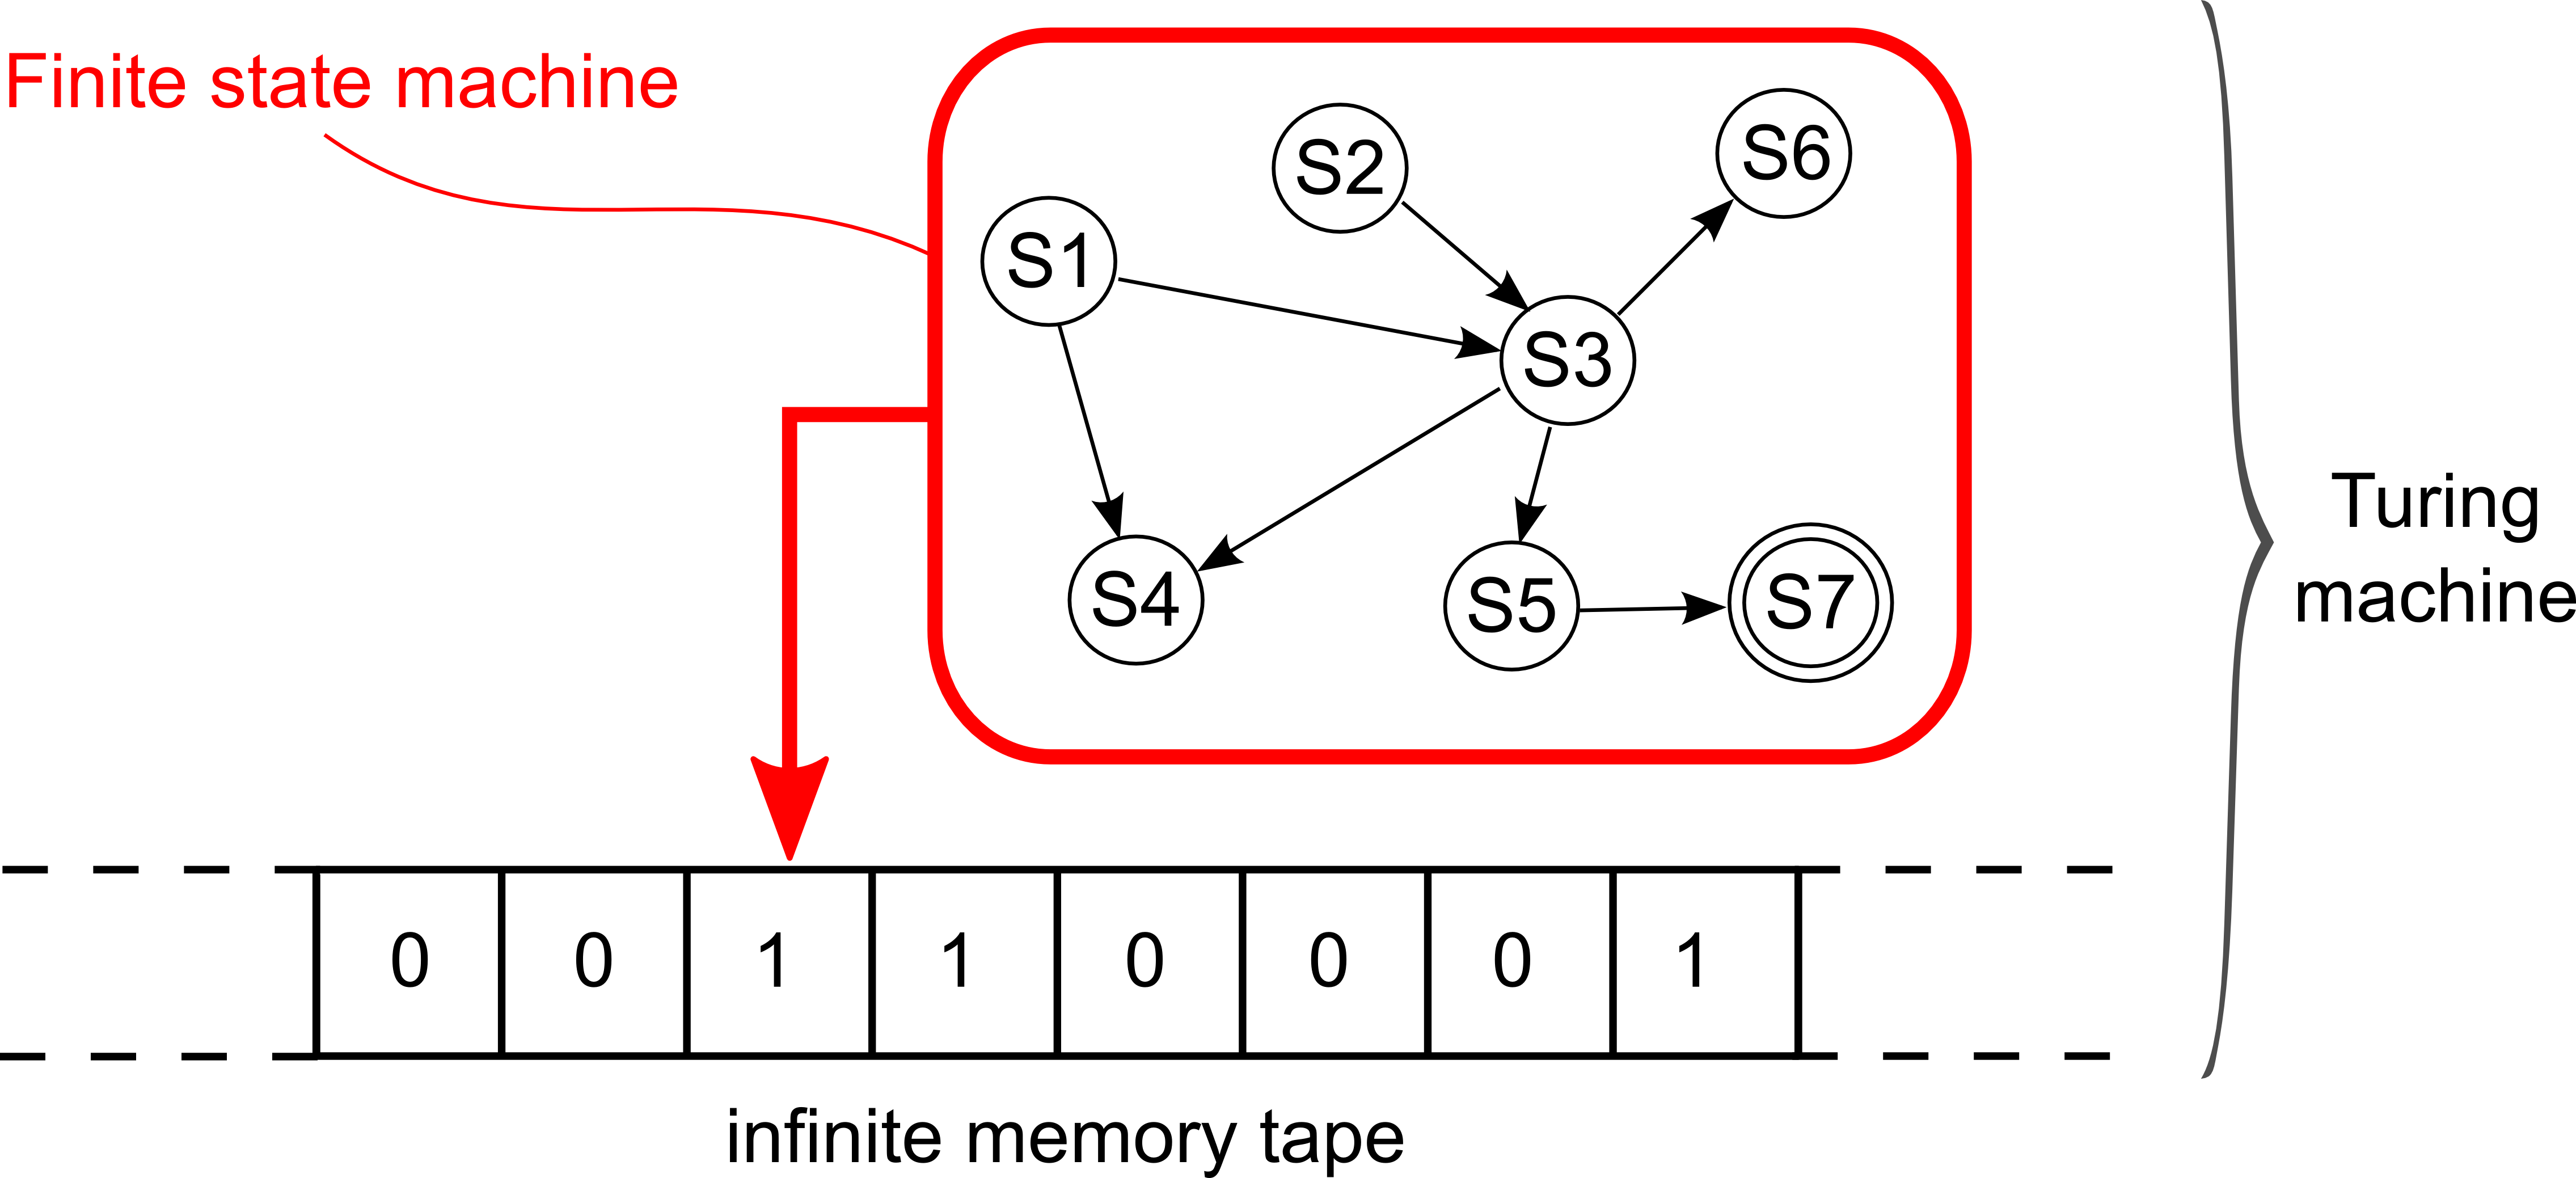
\includegraphics[scale=0.75]{Turing-machine.png}
\end{equation}
所以,深度神经网络 + 记忆~ 就可以变成 universal 的计算器。 如何设计「可微分」的记忆是一个重要课题,因为可微分的记忆可以用 gradient descent 学习。 

% =====================================================================================
\begin{comment}

而很明显,「自由」的 $F$ 算子没有「内部结构」,它能够学习的就像是曱甴那样的、简单的「条件反射」行为。 如果要达到人类的智慧,则要学习很久(到时我们都死了)。

所以问题就是要赋予 $F$ 更多的\textbf{结构},特别是逻辑结构。 直观地说,越多的结构令\textbf{搜寻空间}越小,学习会越快。 这是机器学习里面 inductive bias 的标准做法。

\section{Logic-based AI}

% Strong AI 的问题在理论上已经被\emp{数理逻辑}完整地描述了,馀下的问题是\emp{学习算法},因为在逻辑 AI 的架构下,学习算法很慢(复杂性很高),这就是我们要解决的。

% 我研究 logic-based AI 很多年,因此我的思路喜欢将新问题还原到逻辑 AI 那边去理解,但实际上我提倡的解决办法不是靠经典逻辑,甚至不是 symbolic 的。  但在这篇文章我还是会经常跳回到逻辑 AI 去方便理解。

用数理逻辑 (mathematical logic) 模拟人的思想是可行的,例如有 deduction, abduction, induction 等这些模式,详细可见《Computational logic and human thinking》by Robert Kowalski, 2011.  这些方面不影响本文的阅读。 值得一提的是,作者 Kowalski 是 logic programming,特别是 Prolog,的理论奠基人之一。

在经典逻辑 AI 中,「思考」是透过一些类似以下的步骤:
\begin{eqnarray}
\mbox{前提} & \vdash & \mbox{结论} \\
\boxed{\mbox{今天早上下雨}} & \vdash & \boxed{\mbox{草地是湿的}}
\end{eqnarray}
亦即由一些\emp{命题}(propositions)推导到另一些命题。

推导必须依靠一些逻辑的法则命题 (rule propositions),所谓「法则」是指命题里面带有 x 这样的\emp{变量}(variables):
\begin{equation}
\boxed{\mbox{地方 x 下雨}} \wedge \boxed{\mbox{x 是露天的}} \vdash \boxed{\mbox{地方 x 是湿的}}
\end{equation}
这些法则好比「逻辑引擎」的燃料,没有燃料引擎是不能推动的。

注意: 命题里面的 x,好比是有「洞」的命题,它可以透过 substitution 代入一些实物 (objects),而变成完整的命题。 这种「句子内部」(sub-propositional)的结构可以用 predicate logic (谓词逻辑)表达,但暂时不需要理会这些细节。

「所有人失恋了都会不开心」:
\begin{equation}
\forall z. \; \cancel\heartsuit(z) \rightarrow \frownie{}(z)
\end{equation}
在数理逻辑中这算是一条 \emp{公理} (axiom),但在 AI 中这些公理是从主体的经验中\textbf{学习}出来的,我们仍沿用「公理」这术语。 在 AI 术语中,公理的集合叫 knowledge base,记作 $\KB$。 注意 $\KB$ 是一堆 \textbf{formulas} 的集合。 

Logic-based AI 可以看成是将世界的「模型」压缩成一个 $\KB$: %,里面装著大量逻辑式子
\begin{equation}
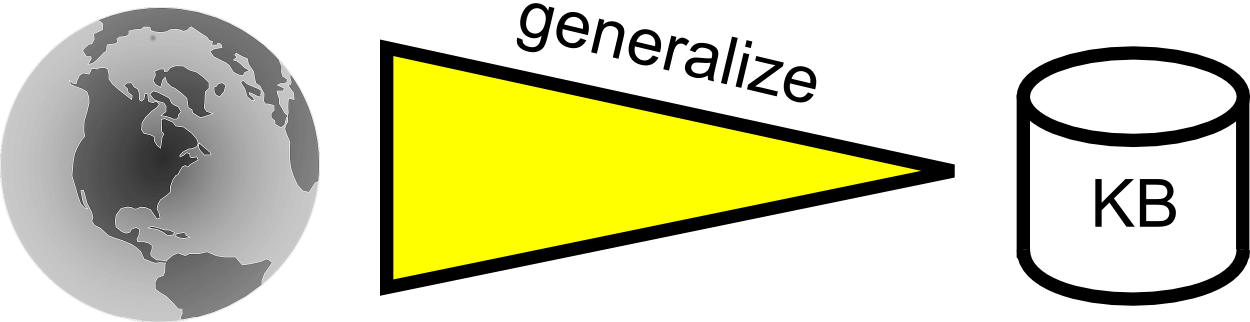
\includegraphics[scale=0.5]{world-model-compression.png}
\end{equation}
世界模型是由大量的逻辑式子经过组合而\emp{生成}的,有点像向量空间是由其「基底」生成; 但这生成过程在逻辑中特别复杂,所以符号逻辑具有很高的\emp{压缩比},但要学习一套逻辑 $\KB$,则相应地也有极高的\emp{复杂度}。

\begin{equation}
x \cup \KB \sdtstile{}{} x'
\end{equation}

\begin{equation}
\KB \, , \, \Gamma \sststile{}{} \Delta
\end{equation}

\end{comment}
% ======================================================================================

\section{什么是 episodic memory?}

在 \cite{Yan2017} 中我们提出了智能系统的 minimal architecture,但这它没有对\textbf{历史}的记忆。 换句话说,只能留意\textbf{当下}发生的事件,但不能记住一段\textbf{故事}。

这牵涉到「什么是记忆?」的问题。 在 minimal architecture 里,$\vect{F}$ 代表 ``static knowledge'',亦即(相对地)\textbf{永恒不变}的知识/规律,而 $\vect{x}$ 代表当下的\textbf{状态}/短期记忆,亦即 ``dynamic knowledge''。  Episodic memory 介乎「长期」与「短期」记忆之间。

在 \textbf{信息处理} (signal processing) 理论中,$z$-transform 以 $z^{-1}$ 可以代表 \textbf{时间延迟} 1 步 (1-step time delay unit)。 用一连串的 $z^{-1}$ 可以组成长度为 $k$ 单位的记忆:
\begin{equation}
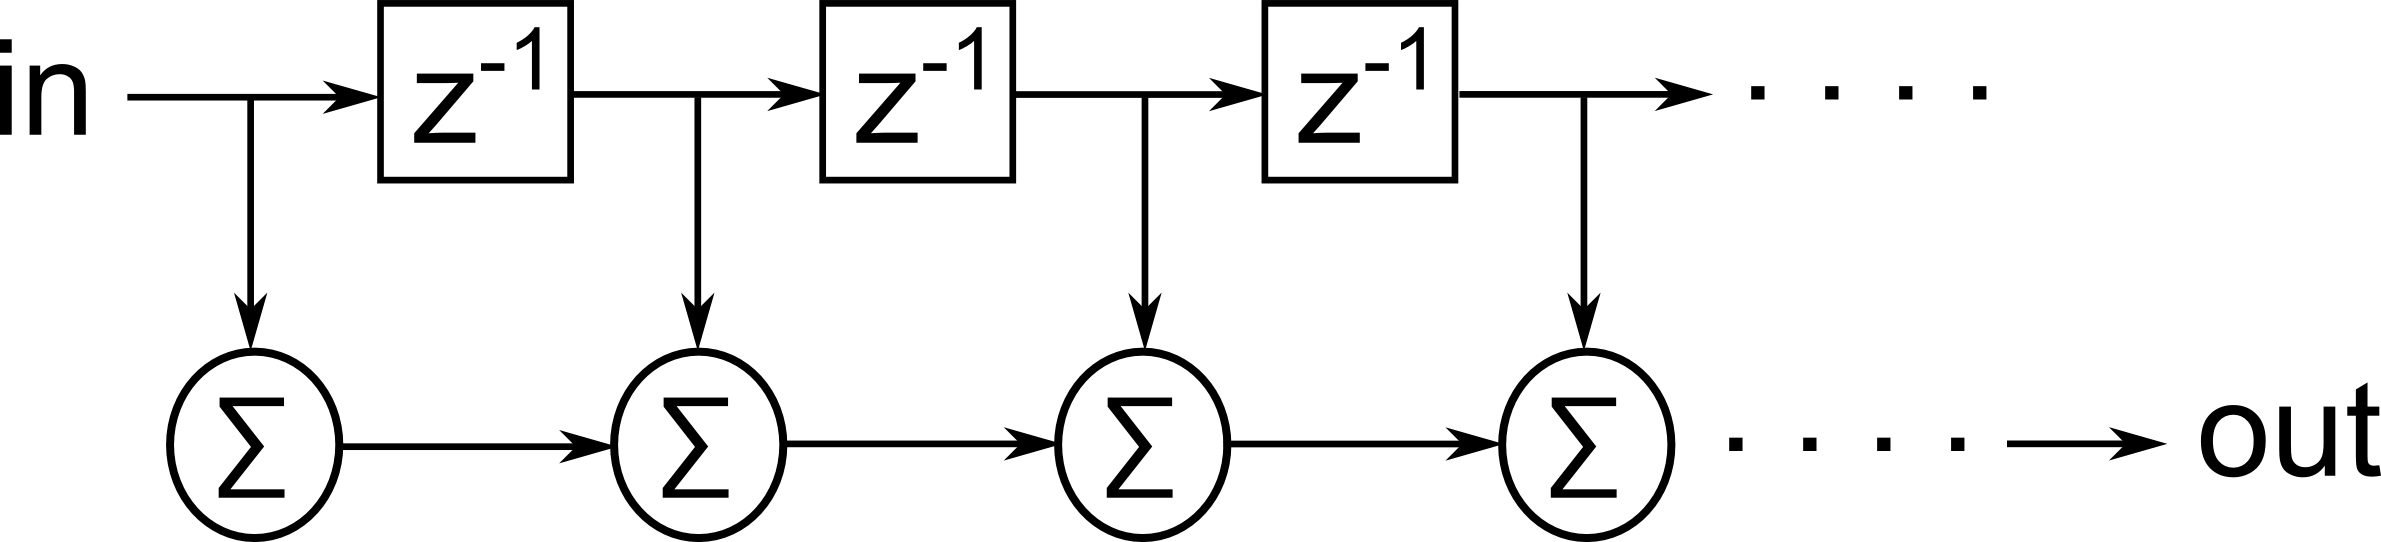
\includegraphics[scale=0.9]{z-memory-0.png}
\end{equation}
以上的无穷串列可以用这个 recursive 结构代替:
\begin{equation}
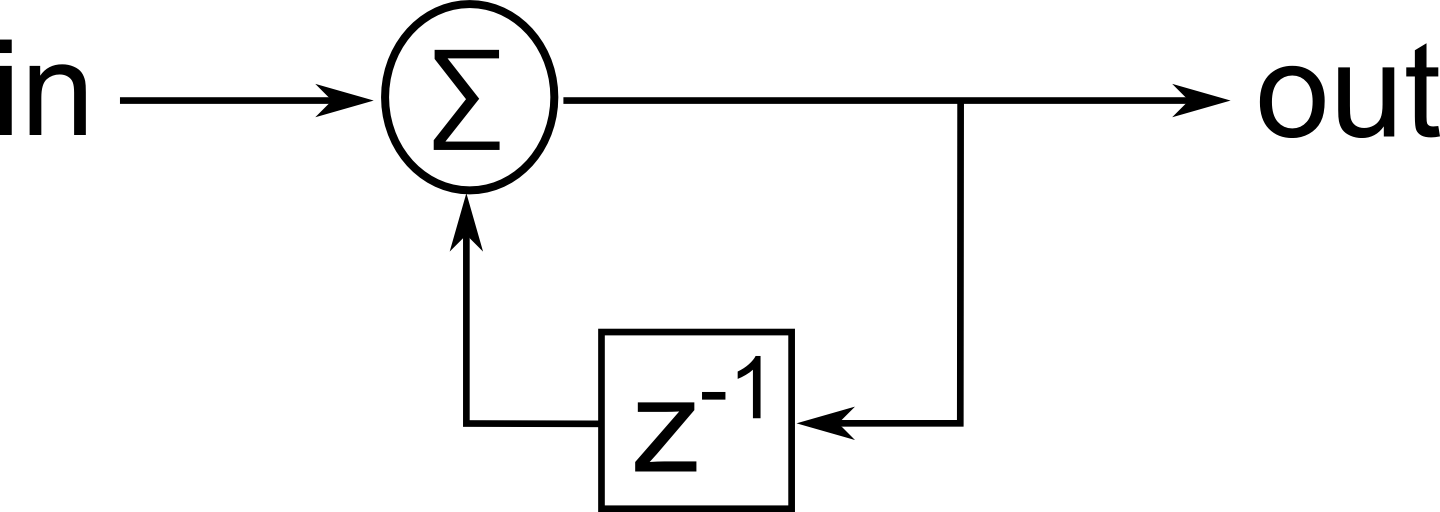
\includegraphics[scale=0.9]{z-memory-1.png}
\end{equation}
多层的 hierarchical 记忆或许可以这样实现:
\begin{equation}
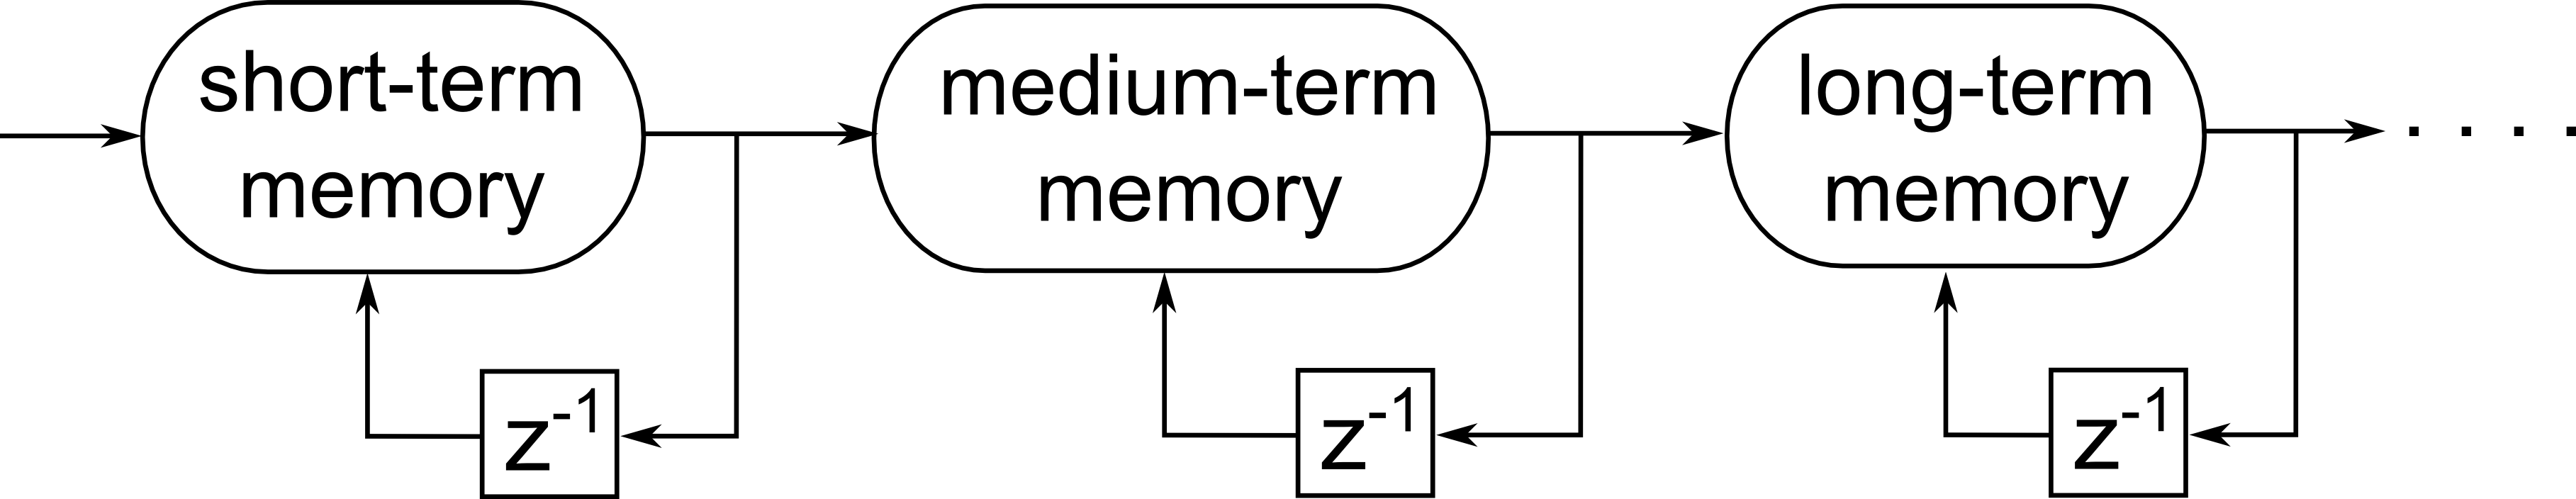
\includegraphics[scale=0.9]{z-memory-3.png}
\end{equation}
%用神经网络实现,可能是这样的:
%\begin{equation}
%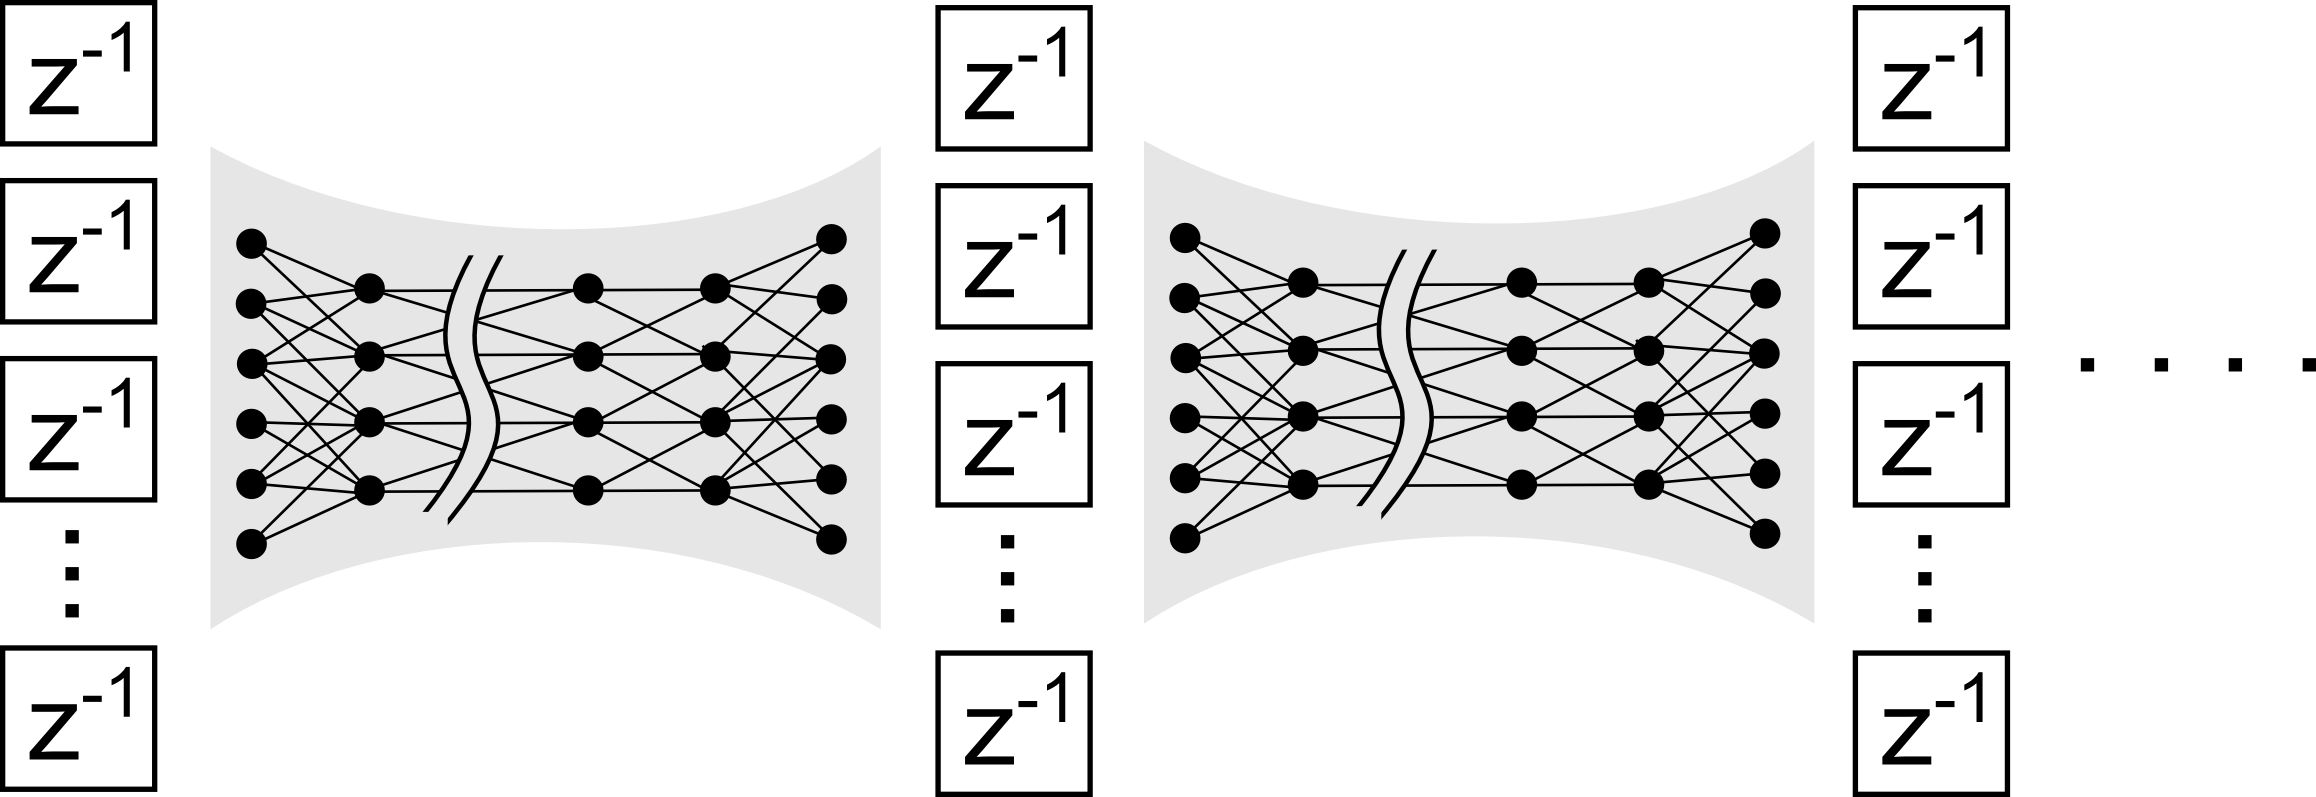
\includegraphics[scale=1.0]{z-memory-2.png}
%\end{equation}
Z-transform 的\textbf{连续时间}版本就是 Laplace transform。

上面的记忆结构来自 Simon Haykin 的经典著作 《Signals and Systems》\cite{Haykin2003}。

\section{Mental state $\vect{x}$ = working memory = 命题的集合}

神经的状态空间由一些 \emp{thoughts}(思维)组成,一个 thought 对应於逻辑中的一条\textbf{命题},例如:
\begin{equation}
\vect{x} = \mbox{ 我正在上课 } \wedge \mbox{ 我很肚饿 } \wedge ....
\end{equation}
这两个 thoughts 是独立的。 也可以有另一个状态:
\begin{equation}
\vect{x}_2 = \mbox{ 我正在搭地铁 } \wedge \mbox{ 我很肚饿 } \wedge ....
\end{equation}
Thoughts 独立的好处是表述的 economy(状态 $\vect{x}$ 分拆成若干独立的 thoughts)。 $\vect{x}$ 是 $M$ 个 thoughts 的集合,$M$ 是 working memory 的大小。 认知科学里有个说法 \cite{}:
\begin{equation}
\mbox{the size of human working memory } \approx 7 \pm 2 \mbox{ items}
\end{equation}
但这些 items 可以有 \emp{chunking} \cite{},例如去超级市场买东西,「意大利粉、茄汁、芝士、香肠」这 4 件东西可以聚合成一个 chunk,这样可以记住的 items 数目多很多。

%思维空间是 $M$ 个 hypercube 的卡积。

\section{记忆 = 状态的历史}

现在回看状态方程:
\begin{equation}
\boxed{\mbox{连续时间}} \quad \quad \dot{\vect{x}} = \vect{f}(\vect{x})
\end{equation}
$\dot{\vect{x}}$ 是状态 $\vect{x}$ 的改变方向,换句话说,这是描述\textbf{状态变化}的方程。 但状态的变化 $\vect{f}(\vect{x})$ 不取决於状态的历史($\vect{x} = \vect{x}|_t$ 仅代表状态在时间 $t$ 的值),所以这个系统没有\textbf{记忆}。 如果想要记忆的话,一个简单的做法是令:
\begin{eqnarray}
\mbox{\color{red} \footnotesize 状态 $\vect{x}$ 的历史} \tikzmark{history} \nonumber\\
\nonumber \\
\dot{\vect{x}} = \vect{f}(\vect{x}|_t, \; \tikzmark{History} {\color{red} \overbrace{\vect{x}(t \in \mathbb{T})}} )
\begin{tikzpicture}[overlay,remember picture]
  \draw[red] (history.center) +(-35pt,-3pt) -- ([shift={(22pt,17pt)}]History.center);
\end{tikzpicture}
\end{eqnarray}
$\vect{f}$ 就是我们的神经网络。 $\vect{f}$ 的输入是:
\let\labelitemi\labelitemii
\begin{itemize}
\item $\vect{x}|_t$ = 当下的状态 = 一些命题的集合; 命题没有 time stamp
\item $\vect{x}(t \in \mathbb{T})$ = 状态的历史; 要考虑每个状态的 time stamp
\end{itemize}

\section{联想记忆 = associative / content-addressable memory}

如果用 content-addressable 的方法,似乎可以不用 time stamps,只要每个记忆 items 之间用「时间先后-link」 连接就可以。 人脑的记忆似乎是这样的。

\section{结论}



% ====================================================================================
\begin{comment}

由一些原始的 sensory data,可以透过逻辑学习出一些 logic formulas,即知识库 (knowledge base) $\KB$。 这个过程叫逻辑\textbf{诱导学习} (inductive logic programming, ILP)。 学经典 AI 的人都知道 ILP,但近数十年来,注意力集中在统计学习,这种符号逻辑的学习法被忽视。 

原始的 sensory data 可以透过神经网络进行模式识别,也可以透过 ILP 进行模式识别,两条路径的结果很明显应该是(近似地) isomorphic 的:
\begin{equation}
\begin{tikzcd}[]
\mbox{Logic representation} \arrow[rr, phantom, "\simeq"] & & \mbox{Neural representation} \\
& \arrow[ul, "\mbox{inductive logic learning}"] \arrow[ur, "\mbox{deep NN learning}" swap] 
\includegraphics[scale=0.5]{sensory-data.png} &
\end{tikzcd}
\end{equation}
但实际上,这两边的 $\rightarrow$ 都是 \textbf{资讯压缩} 的过程,因此是\textbf{不可逆}的,所以中间的 $\simeq$ 未必成立。 (如果是可逆的,我们可以从一边往下回到原始资料然后再往上去到另一边。)

%我以前花了很多时间思考怎样将逻辑的 representation 过渡到神经网络去,但发觉这个目标非常 elusive。

%一方面,逻辑是几百年来发展起来的关於人类思考的规律; 逻辑的描述是正确的; 逻辑和神经之间必然有一个 correspondence,因为它们都在做同样的事(智能)。 

在\textbf{认知科学}里,有很多人相信大脑的内部的 representation 是一些所谓 ``mental models'',而很少人会相信大脑使用一些像命题那样的符号结构做 representation,甚至用 $\lambda$-calculus 那样的符号 manipulation 去思考。

举例来说,用文字描述一起凶杀案,读者心目中会建立一个「模型」,它类似於真实经验但又不是真实的。 人脑似乎是用这样的 mental models 思考,而不是一些命题的集合。 有两本论文集关於 model-based reasoning,基於逻辑的: \cite{Magnani1999} \cite{Magnani2002}。
%至於 mental models 是什么,目前认知科学还未有定论。

我终於发现到,logic-neuro correspondence 必须透过 model theory才能达成:
\begin{equation}
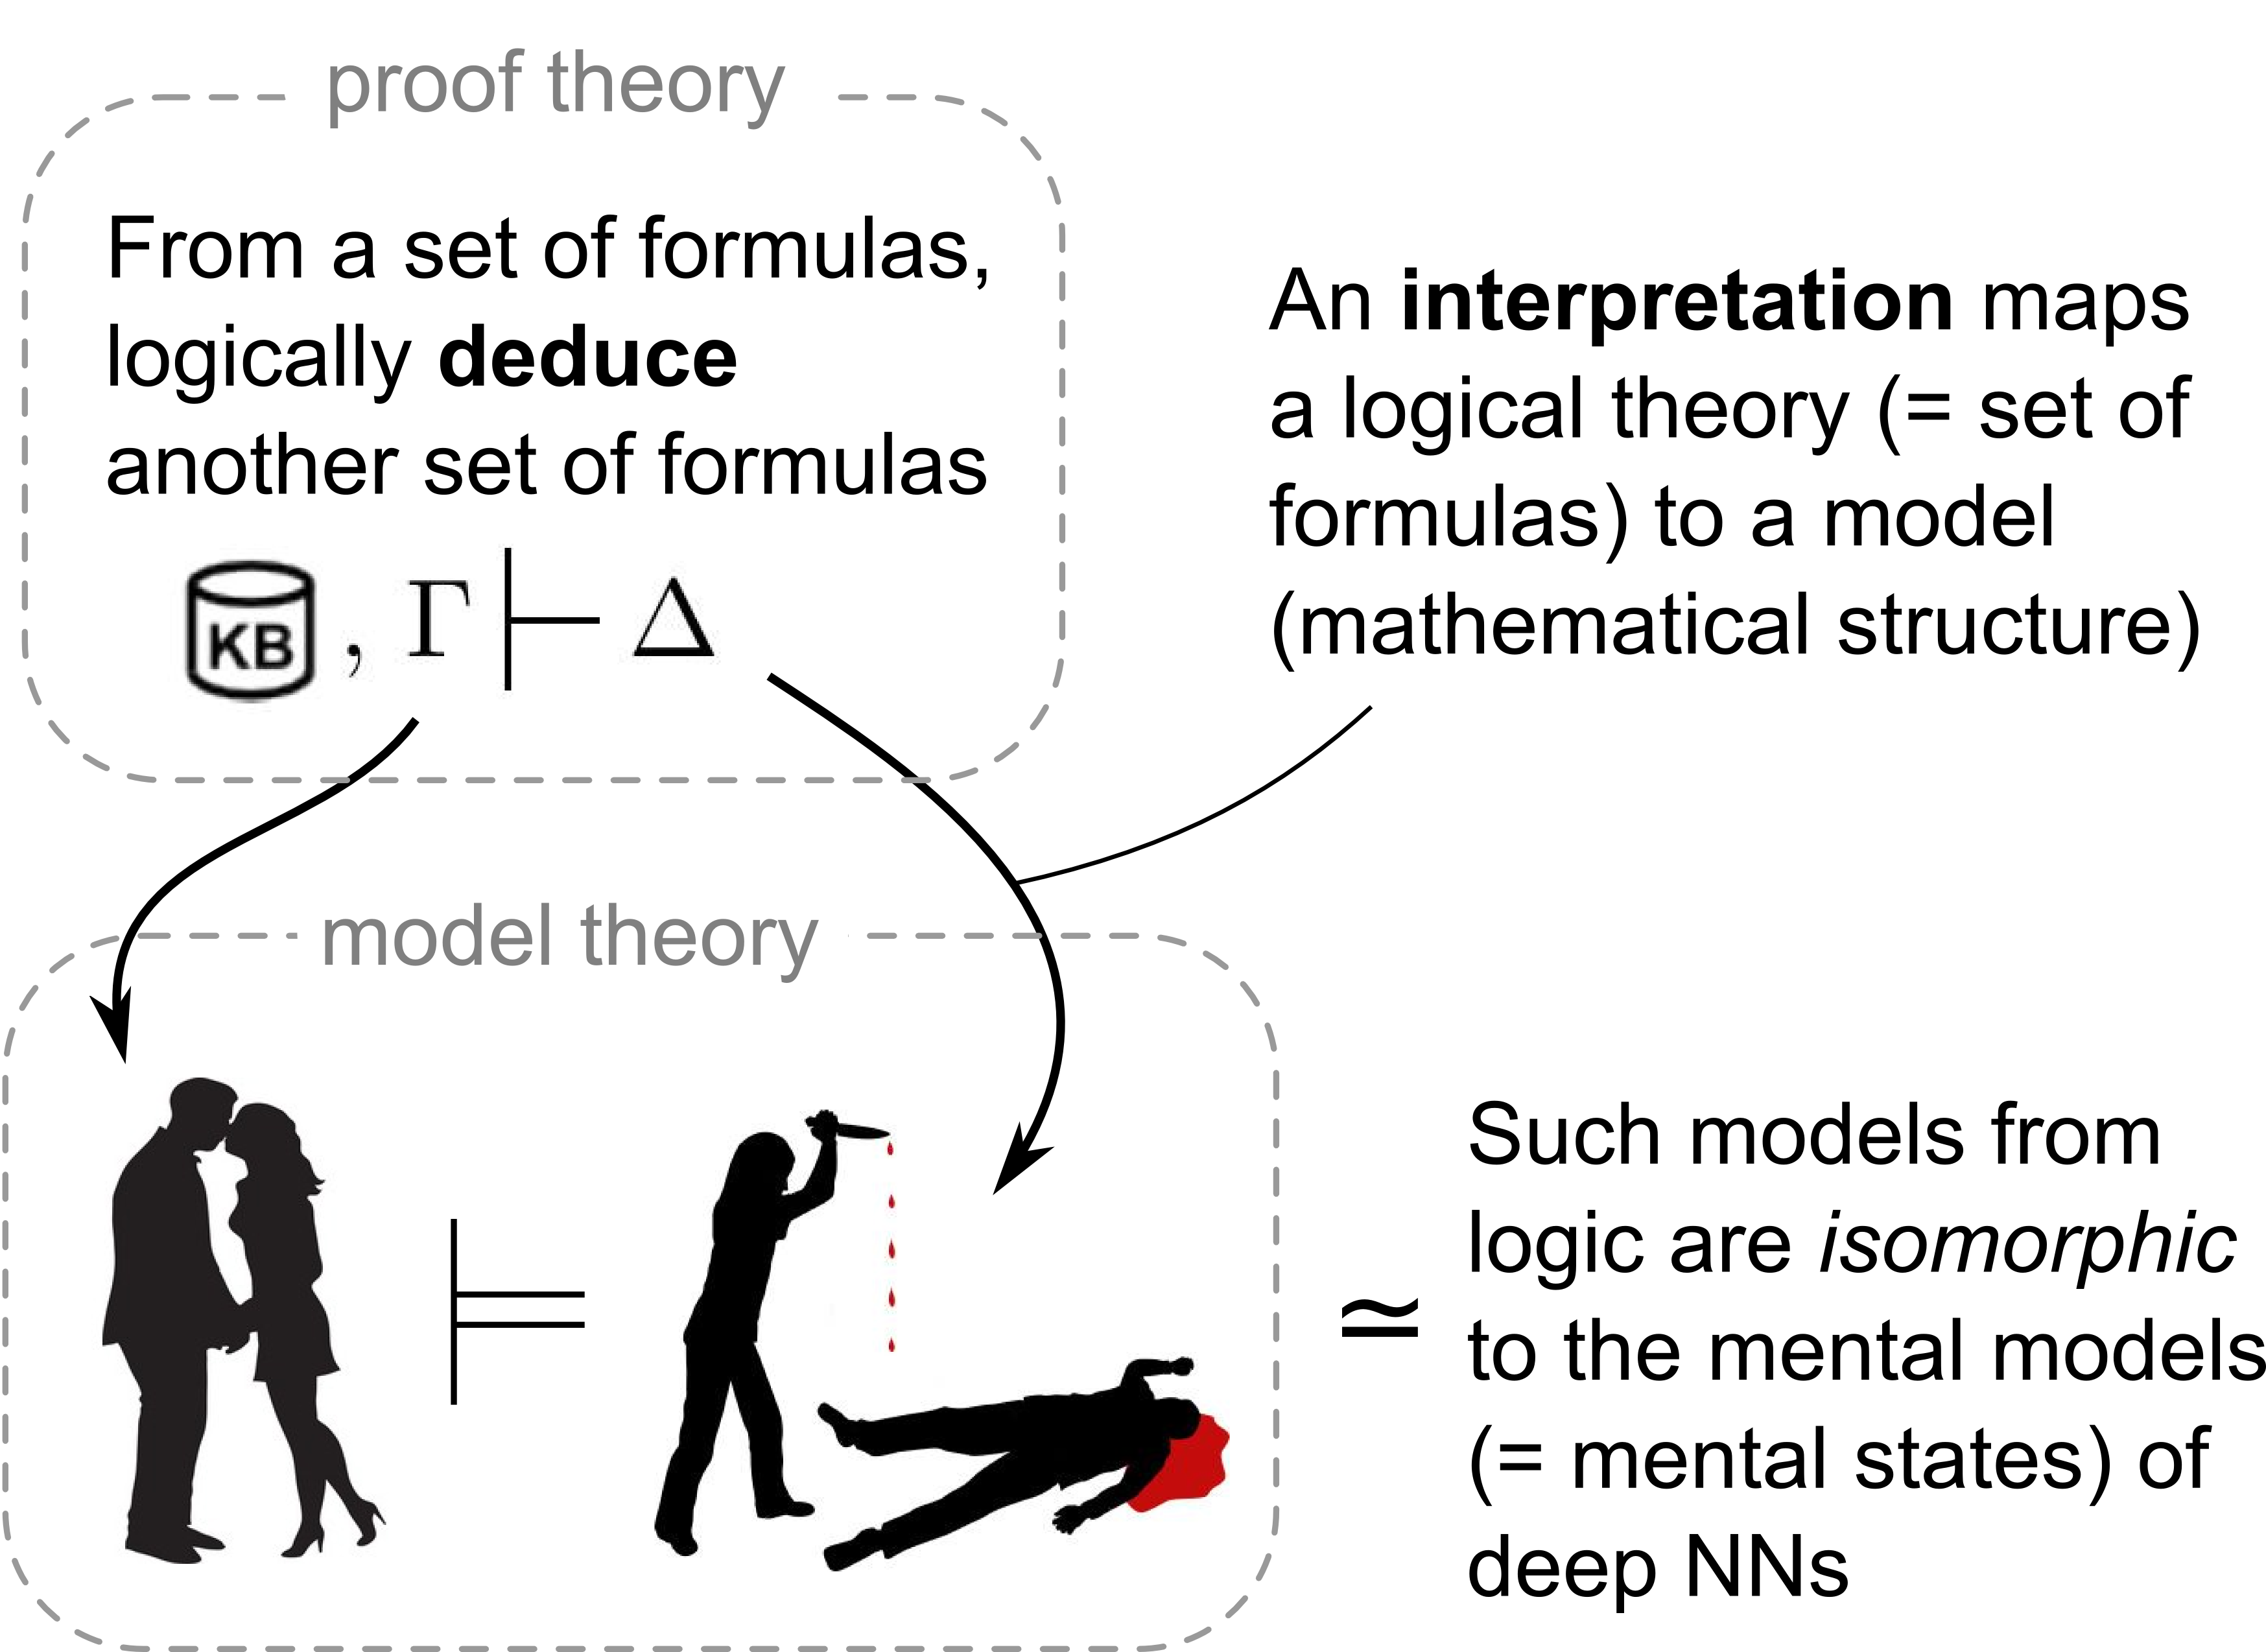
\includegraphics[scale=0.75]{model-theory.png}
\end{equation}

$\vdash$ 是指由一些(符号逻辑的)\textbf{命题集合}推导出新的命题集合。 $\vDash$ 指的是,由一个\textbf{模型}推导出另一个模型必然为真。

% \footnote{Knowledge-based model construction (\textbf{KBMC}) 这个术语较少人知道,但其实是最关键的结构; 换句话说,就是从 $\KB$ 中抽出一组命题 $\Gamma$,去\textbf{组合}一个 model 或 proof tree,而这个 proof tree 的某个节点,就是新的结论。 亦即 $\Gamma \vdash Q$。 KBMC 的概念适用於经典逻辑也适用於 Bayesian networks。}

\subsection{由一些命题推导出另一些命题}

命题也有内部结构(即命题可以由概念原子组合而成),但我们先从最简单情况谈起,即\textbf{命题逻辑}。

最简单的经典命题逻辑,是 Boolean propositional logic,它的\textbf{代数形式}是我们熟悉的 Boolean algebra,二者几乎没有分别(纯粹逻辑符号和代数符号的对应)。 

在 Boolean algebra 可以定义一种 ideal $I$:
\begin{itemize}
\item If $a, b \in I$ then $a \wedge b \in I$
\item If $a \in I$ and $a \le b$ then $b \in I$
\end{itemize}
其中 $a \le b$ 表示 $a \Rightarrow b$(a 蕴涵 b)。

由上面可以看出,这个 ideal 其实是由某些元素(命题)生成的 \textbf{逻辑后果}(logical consequence); 换句话说,给定一个命题集 $\Gamma$,问 $\Gamma \stackrel{?}{\vdash} a$(从 $\Gamma$ 可以推导出 $a$ 吗?) 就等於问 $a$ 是不是 $\Gamma$ 生成的 ideal membership 问题。 也可以说,代数 ideal $\equiv$ 逻辑 consequence。 (严格来说,consequence 对应的是 filter 的概念,而 filter 是 ideal 的 dual,因为 0 和 1 对应的倒错,但这不是重点。)

\textbf{逻辑后果}可以记作 $\vdash$ 或 Cn,Tarski 定义了 $\vdash$ (很明显)的特性:
\begin{itemize}
\item (reflexivity): \quad $A \vdash A$ for every formula $A$
\item (monotonicity): \quad $A \vdash Q$ implies $A, B \vdash Q$
\item (`cut'): \quad \quad $A \vdash B$ and $A, B \vdash Q$ implies $A \vdash Q$
\end{itemize}

% 在 Boolean algebra 中有一些 inference rules,例如:

以上是 Boolean logic 的代数化,但如果考虑 probabilistic logic 就更为复杂,需要用到 Bayesian networks,而 filter $\equiv$ consequence 的原理似乎不再适用。 

Bayesian network 的细节很麻烦,可以花整个研究生课程来讲。

重点是: Bayesian network 是由一些\textbf{条件概率} (conditional probability) 的关系生成的。 每个\textbf{节点}是一个命题,每个\textbf{连结}是一个条件概率关系,例如:
\begin{equation}
P(A|B,C,D,...) = \vec{p}
\end{equation}
其中 $\vec{p}$ 是一个 conditional probability table (CPT)。

对不起,用一个较粗俗的例子说明(在我多年的教学经验里,这是最易懂的例子):
\begin{equation}
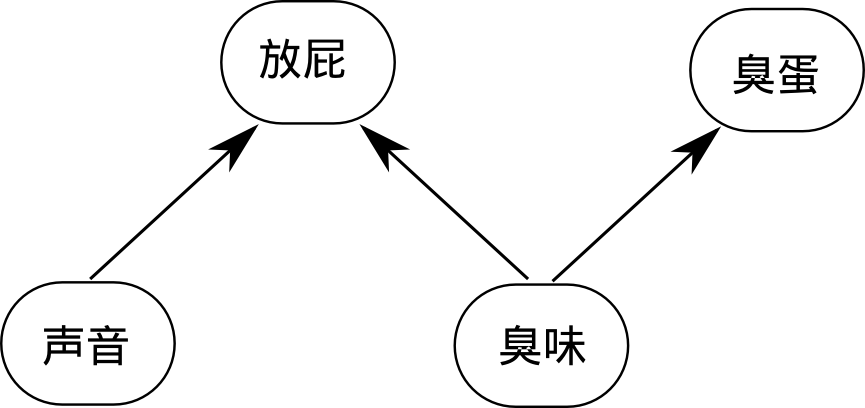
\includegraphics[scale=0.5]{farting.png}
\end{equation}
这个 Bayesian network 是由两个 CPT 生成的:
\begin{eqnarray}
P(\mbox{放屁} | \mbox{臭味}, \mbox{声音}) = \vec{p}_1 \nonumber \\
P(\mbox{臭蛋} | \mbox{臭味}) = \vec{p}_2
\end{eqnarray}
如果有「声音」又有「臭味」,则「有人放屁」的机率很高,而「臭蛋」的机率却会减少。 换句话说,「臭蛋」的机率被扯到「放屁」那边去了; 这个现象叫 ``explaining away'',它说明 Bayesian network 中,所有节点都是 globally 相关的。 所以,当求解 Bayesian network 的某个节点时,它的概率会是一连串很复杂的 sum-product 形式。 看来用 Bayesian network 表示 $\vdash$ 的方法太复杂了。

可幸的是,可以用 Monte Carlo 方法求解 Bayesian network: 开始时随机地指定节点的概率,然后随机地选取某些节点来作「\textbf{局部}」的 update; 当随机 update 的次数趋近无限,节点的机率会收敛到正确的值。 换句话说: 这是一个 \textit{local} 的计算 Bayesian network 的方法。

\section{模型论}

模型论基础可参看 \cite{Doets1996} \cite{Manzano1999}。 模型论的做法是将逻辑的符号\textbf{语言} (language $\mathcal{L}$) 和它所指涉的\textbf{结构} $\mathcal{L}$-structure 分割,中间用 interpretation map 关联起来。

$\mathcal{L}$ 就是符号的集合 (predicates, relations, functions, constants),递归地生成出句子和复合句子。 这些都是 symbolic 的东西。

$\mathcal{L}$-structure 可以是任何抽象代数结构,它通常包含一个 base 集合,然后在集合上定义一些函数和关系。 

模型论的中心思想是透过 interpretation $i$ 去「保存」一些关系,例如:
\begin{equation}
R(a,b) \stackrel{i}{\mapsto} R^\mathbb{M}(a^\mathbb{M}, b^\mathbb{M})
\end{equation}
$R$ 是一个关系,$x^\mathbb{M}$ 代表在结构 $\mathbb{M}$ 之上,$x$ 所对应的物体。 左边是符号逻辑,右边是实体的结构。 模型论应用在 first-order logic,得出 $\vdash$ 和 $\vDash$ 等价的结论(看起来就好像同语反覆),这在数理逻辑教科书中都有,例如 \cite{Hedman2004}。 

如果用範畴论的方法表示逻辑结构和神经结构之间的对应:
\begin{equation}
\begin{tikzcd}[]
\mathcal{L} \arrow[d, "i"] \\
\mathbb{M} \arrow[r, phantom, "\simeq"] & \mathbb{X} \\
& \arrow[u, "\mbox{deep NN}" swap] \mathcal{S}
\end{tikzcd}
\end{equation}
\renewcommand\labelitemi{\textbullet}
\begin{itemize}
\item $\mathcal{L}$ = category of logic theories (= sets of formulas)
\item $i$ = interpretation maps
\item $\mathbb{M}$ = category of models (from logic)
\item $\mathbb{X}$ = category of models (from deep NNs)
\item $\mathcal{S}$ = sensory input
\end{itemize}

上图等同於下面的卡通解释:
\begin{equation}
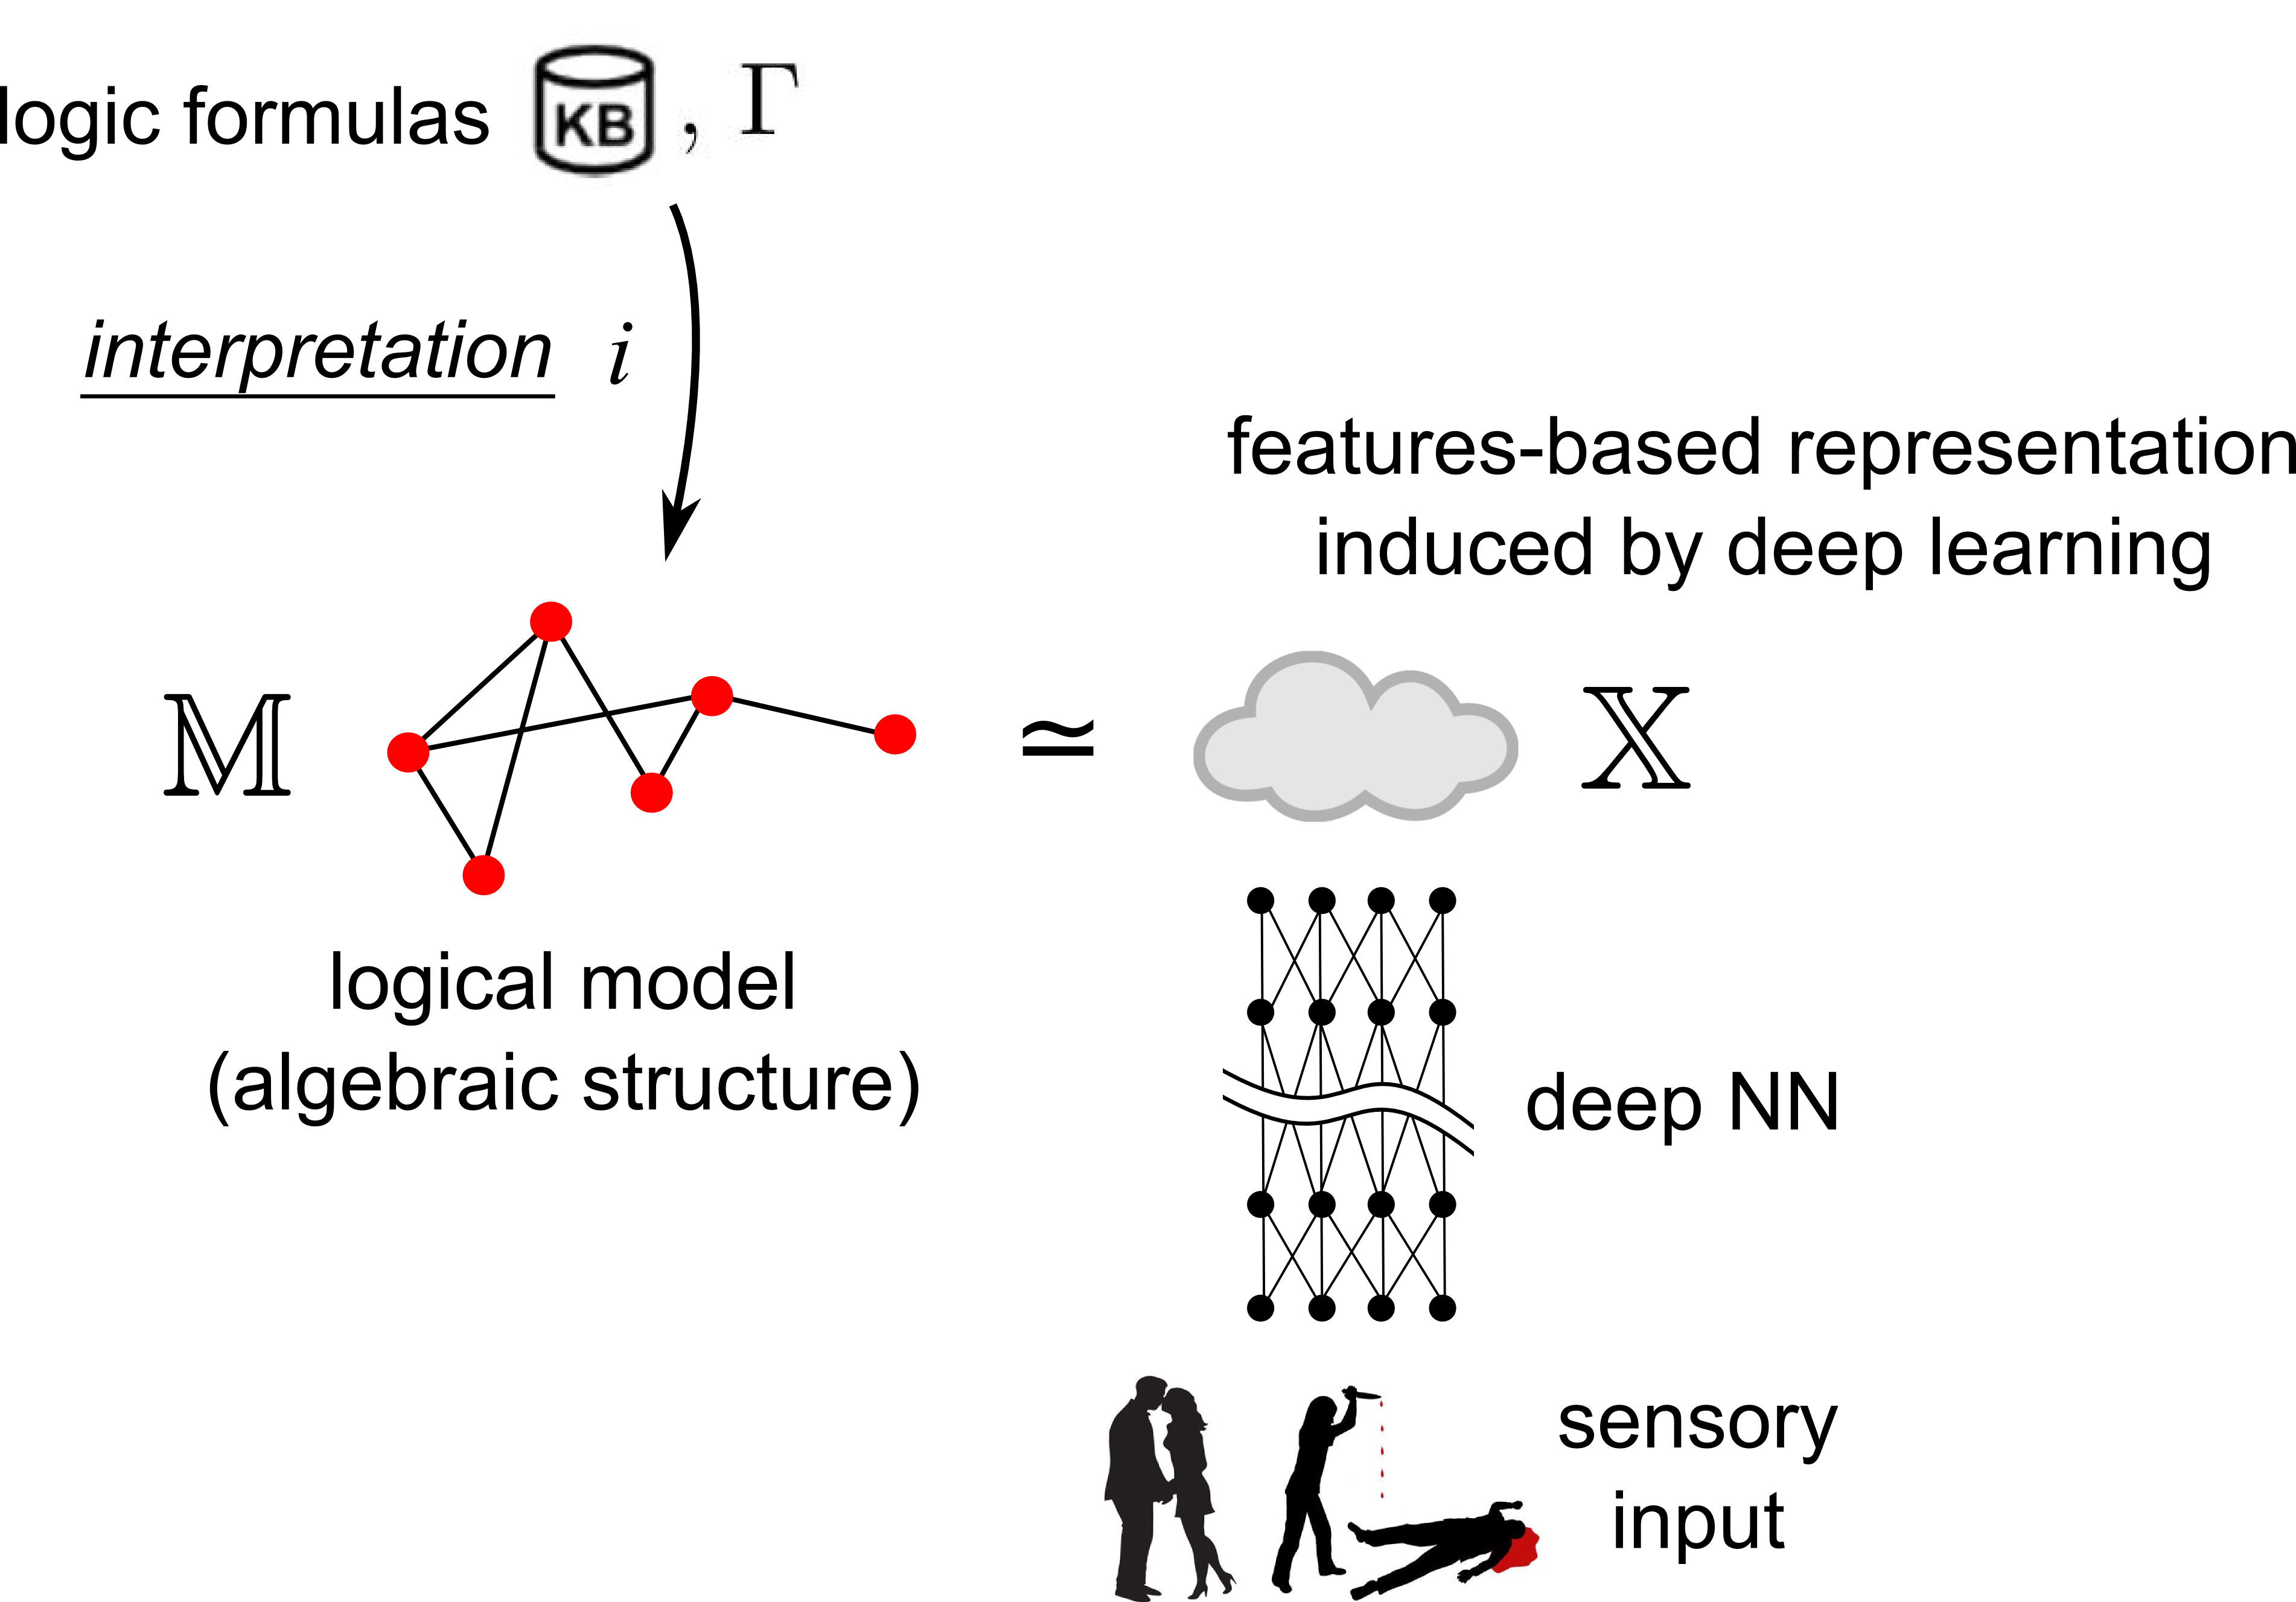
\includegraphics[scale=0.7]{model-theory-cartoon.png}
\end{equation}

换句话说,$\mathbb{X} = \vcenter{\hbox{
\includegraphics{cloud.png}}}$ 是由深度学习 induce 出来的结构; 但它的结构对我们来说是不透明的(这是神经网络的弱点)。

而 $\mathbb{M} = \vcenter{\hbox{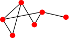
\includegraphics{algebraic-model.png}}}$ 的结构就是模型论研究的对象。
%是 free 的; 换句话说,那 $i$ map 的 source domain 是固定的,但 target domain 是自由的。 这导致 $i$ map 的学习很困难,因为 $\mathbb{M}$ 和 $\mathbb{X}$ 的结构都不清楚。 必须更详细分析 $\mathbb{M}, \mathbb{X}$ 的结构。

%\section{模型论和 interpretation 的结构}

在模型论中,$\mathcal{L}$ 是逻辑句子的範畴,$\mathbb{M} = \vcenter{\hbox{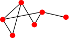
\includegraphics{algebraic-model.png}}}$ 可以是任何抽象代数结构。 只需把 $\mathcal{L}$ 中的 constants, predicates, relations, functions 映射到 $\mathbb{M}$ 就行。 为简化讨论,我们只考虑 constants 和 relations,因为二者是逻辑中最\textbf{本质}的东西。 
\begin{eqnarray}
\mathcal{L} & \quad \stackrel{i}{\rightarrow} \quad & \mathbb{M} \nonumber \\
\mbox{constant symbol} & \quad \stackrel{i}{\mapsto} \quad & \; 
\includegraphics[scale=0.5]{node.png} \\
\mbox{relation symbol} & \quad \stackrel{i}{\mapsto} \quad & \; 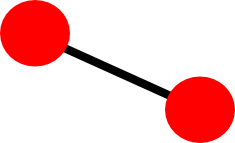
\includegraphics[scale=0.5]{link.png} \nonumber
\end{eqnarray}

问题是在神经那边缺乏 $\vcenter{\hbox{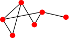
\includegraphics{algebraic-model.png}}}$ 的结构。 一直以来,人们习惯把神经网络看成是 ``black box'',但如果我们不知道 $\mathbb{X} =  \vcenter{\hbox{
\includegraphics{cloud.png}}}$ 的结构,就无法建立 $\mathbb{M} \simeq \mathbb{X}$ 的 isomorphism。

\section{结论}

但要注意的是这对应未必是一对一的,可能是一个 constant 对应几个 neurons 的(线性?)\textbf{组合}。 具体情况可能像以下的示意图(实际上每层神经网络可能有很多神经元):
\begin{equation}
\label{conclusion2}
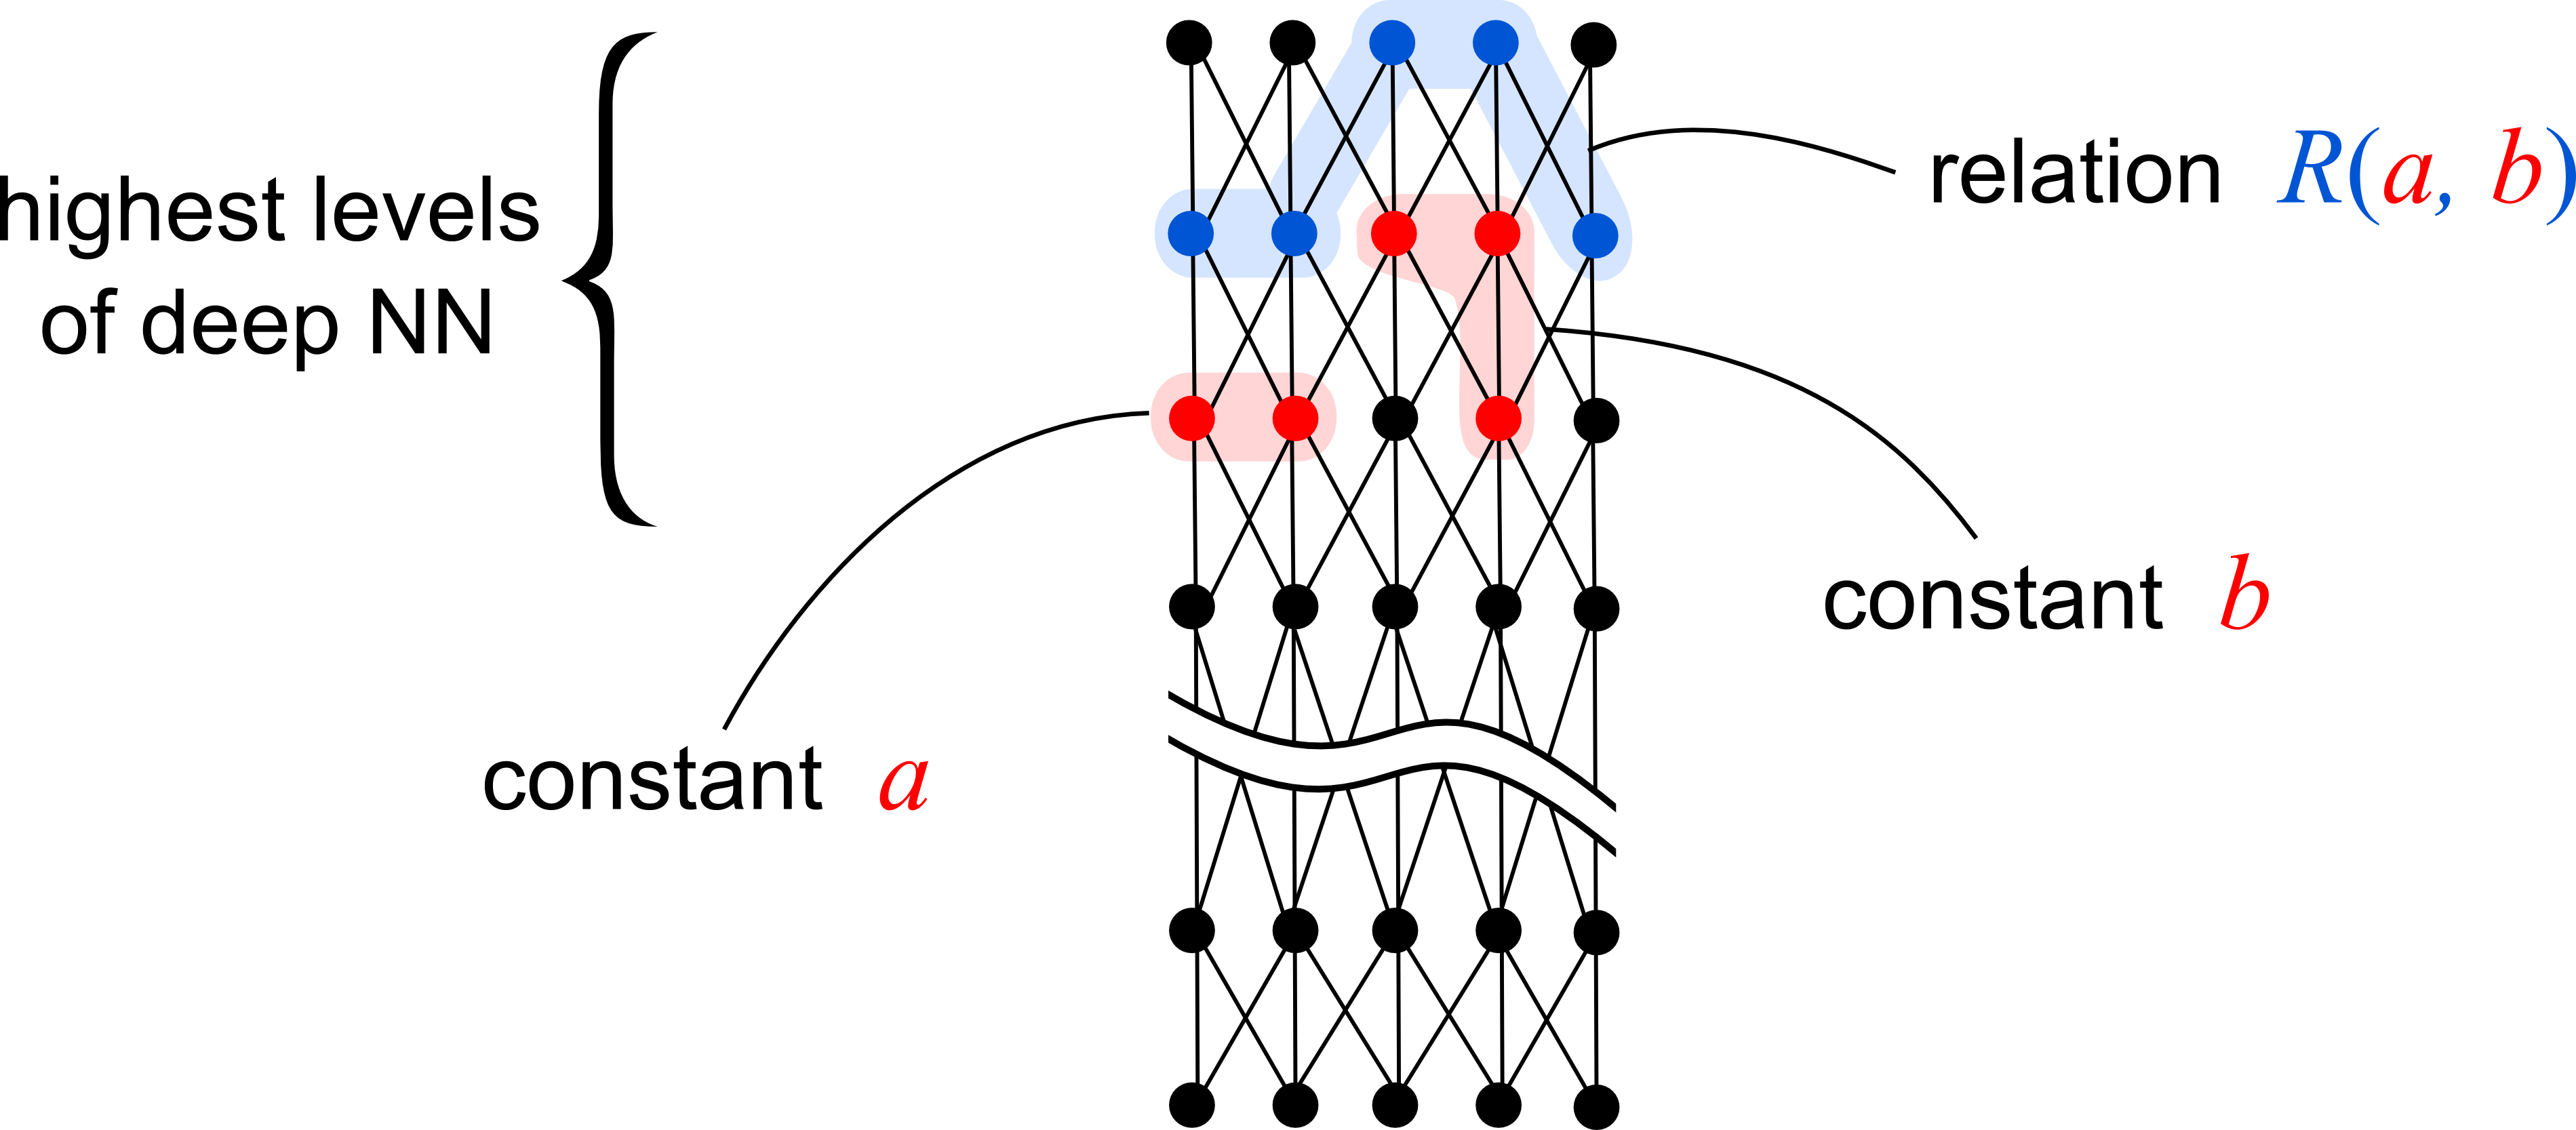
\includegraphics[scale=0.5]{actual-bridge.png}
\end{equation}
$R(a,b)$ 可以在 $a, b$ 的 common parents 中寻找(例如那些蓝色神经元,$R(a, b)$ 的值 = 蓝色神经元的某个线性组合)。  验证的方法是: 当 $a$ 和 $b$ 的信号都是「有」时,$R(a, b)$ 的值也应该是 true。 


这篇论文并不太成功,因为跳到 (\ref{conclusion1}) 和 (\ref{conclusion2}) 的结论没有严谨的根据,只是直观上觉得有可能。 理论上来说,既然知道了 $\mathbb{M}$ 那边是怎样生成的、$\mathbb{X}$ 那边是怎样生成的,则要在两边建立「高速公路」应该是可行的。 实际上,似乎只要建立一个深度网络就可以,因为神经网路是 universal function approximator,根本不用考虑 $\mathbb{M}$ 和 $\mathbb{X}$ 这两个结构之间的关系。

进一步的研究,希望数学专业的人能帮助一下:
\begin{enumerate}
\item 在逻辑那边,可不可以转换成 algebraic geometry 的结构? 即是说: 逻辑式子 $\simeq$ 代数方程。 这种代数逻辑的做法,我暂时只知道有 \cite{Andreka2001},是很偏门的研究。
\item 能不能根据 $\mathbb{M}$ 和 $\mathbb{X}$ 的结构,找出它们之间的桥的最简单形式?  可以用数学归纳法,逐步考虑 $\mathbb{M}$ 和 $\mathbb{X}$ 生成的方式,或许有帮助?
\end{enumerate}

%看上去颇复杂,但这样已经可以直接由逻辑式子 $\mathcal{L}$ 映射到深度网络的输出层。  在未有这理论之前,完全不知道这个 map 的结构;  但现在假如理论是正确的话,只需要简单的组合搜索 (combinatorial search) 就可以找到对应。  

应用: 对於用深度学习做 natural language understanding 的人,这理论或许会很有用。 

% Armed with this theory, we may construct an actual neuro-logic bridge.

\section{Prior art}

\begin{itemize}
\renewcommand\labelitemi{\textbullet}

\interfootnotelinepenalty=10000

\item Bader, Hitzler, H\"{o}lldobler and Witzel 在 2007 年提出了一个 neural-symbolic integration 的做法 \cite{Bader2007}。 他们首先由 logic theory 生成抽象的 Herbrand model\footnote{Herbrand model 是邏輯 AI 中常用的概念,大意是用邏輯語言 $\mathcal{L}$ 生成「所有可以代入的東西」(instantiating whatever that can be instantiated),由此產生的不含變量的句子 (sentence) 的集合。 換句話說,Herbrand model 的特點是它只靠 $\mathcal{L}$ 自身產生它的模型,而不依賴任何外在結構。 每个邏輯 theory 都必然至少有一个 Herbrand model。},再将 Herbrand model 映射到某个 fractal 空间,然后直接用神经网络学习那 fractal 空间。  虽然用了 model theory,但他们没有利用到本文所说的 $\mathbb{M}$ 和 $\mathbb{X}$ 之间的关系。 

\item Khrennikov 在 1997 年开始的多篇论文中提出了用 $p$-adic 代数来模拟思维空间 $\mathbb{X}$ 的结构,详见\cite{Anashin2009} 一书。 一个 $p$-adic 数可以看成是一个 $p$ 进制的小数,$p$ 是任何质数。

\item 经典逻辑是二元逻辑,近代已经有无数将它扩充到 fuzzy 或 probablistic 的尝试(作者也提出过 \cite{Yan2012}),但仍未有统一的理论。 与此不同的另一个方向,如果将点看成是 first-order objects,谓词是点空间上的函数,直接得到 metric structures 上的连续逻辑 (continuous first-order logic) ~ \cite{Yaacov2008},这可以看成是一种 $\mathbb{M}$ 的结构。

\item 模型论中有(超滤子)ultra-filter 和 ultra-product 这些建构,它们起源於泛函分析,最近有很多横跨模型论和 Banach 空间的新研究 \cite{Iovino2002}。 简单地说 ultra-product 用来将一些 models 构造出新的乘积 models。 但我粗略地看过一下之后发现 ultra-product 通常涉及无穷集合,而且是很大的物体,在计算机上应用似乎不太实际。

\end{itemize}

\section{逻辑变量的处理}

这可能是最辣手的部分。

Alfred Tarski 提出了 cylindrical algebra 来解决「一阶谓词逻辑」的变量问题,但据说 Tarski 自己也觉得 cylindrical algebra 「不好用」。 我觉得它比较难明,从略。

个人觉得比较好的做法是 Paul Halmos 的 algebraic logic。 其中最关键的建构是:
\renewcommand\labelitemi{--}
\begin{eqnarray}
\mbox{谓词} : \mbox{物体} & \rightarrow & \mbox{命题空间} \nonumber \\
\cancel\heartsuit : \cancel\heartsuit(\mbox{john}) & \mapsto & \mbox{「阿 John 失恋」} \nonumber \\
\cancel\heartsuit : \cancel\heartsuit(\mbox{pete}) & \mapsto & \mbox{「阿 Pete 失恋」}
\end{eqnarray}
换句话说,predicate(谓词)就是一些将 object (逻辑中的物体,或「常项」,constants)映射到个别命题的\textbf{函数}。 这些谓词函数可以有一个或多个\textbf{参数},分别叫 monadic 和 polyadic predicate calculus。

最新的逻辑代数化方法来自\textbf{範畴论},William Lawvere 在 1960's 年代提出(也就是 \textit{Conceptual Mathematics} 这本书的作者之一)。  他发现了 $\forall$ 和 $\exists$ 是 adjoint functors 的关系; 这个 adjunction 比较难懂,有兴趣可以看 \cite{Lawvere2003}。
\end{comment}
% =====================================================================================

\bibliographystyle{plain} % or number or aaai ...
\bibliography{AGI-book}

\end{document}
% ***************************************************************************************

\section{关於逻辑....}

由初始状态 $x$ 过渡到 $x'$:
% \mathrm{L}
\begin{equation}
x \sststile{}{\KB} x'
\end{equation}
注意 $x, x'$ 是命题的\textbf{集合},$x, x' \subset \mathcal{P}(\mathcal{L})$,the power set of all logic formulas。

所谓 $Q$-value 其实是在 $X \times U$ 空间上的\textbf{能量分布}; $(x,u) \mapsto Q$。 意思是说: 在状态 $x$ 执行动作 $u$,其价值是多少? (因为我们等同了价值和能量。)  也可以说,$Q$ 是 $X \times U$ 上的一个\textbf{测度} (measure)。

我们将逻辑推导中的\textbf{搜寻}纳入到 transition function 的功能之中。 换句话说,transition function 的功能并不只是推导; 它是一种类似 stochastic search 的「游荡」。   

在逻辑 AI 这边,我们要计算的是分布在 $\sststile{}{\KB}$ 上的测度 $Q$; 换句话说,对於不同的 $\KB$,我们有不同的 $\vdash$。 这似乎等於分布在所有不同的 $\KB$ 上的测度。

In LBAI the knowledge representation structure is built (\textit{fixed}) from the bottom up:
%\begin{equation}
%\mbox{words } \triangleright \mbox{ sentences } \triangleright \mbox{ logical form } \triangleright \mbox{ logical KB}
%\end{equation}
%Thus the structure of the KB is \textit{fixed} by the human designer. % This rigidity is perhaps why learning in logic-based systems is slow.

% In natural language, an idea can be expressed as a concatenation of words, for example:\\
% And it is just a short jump from word concatenations to symbolic logic.  But this jump may land us into a logic-based ``tar pit'', in which everything is theoretically possible, but often too slow in practice.

%It is just a short jump from the expression of ideas as word concatenations to logical form as linear (or tree-like, or graph-like) compositions of symbols:
\begin{equation}
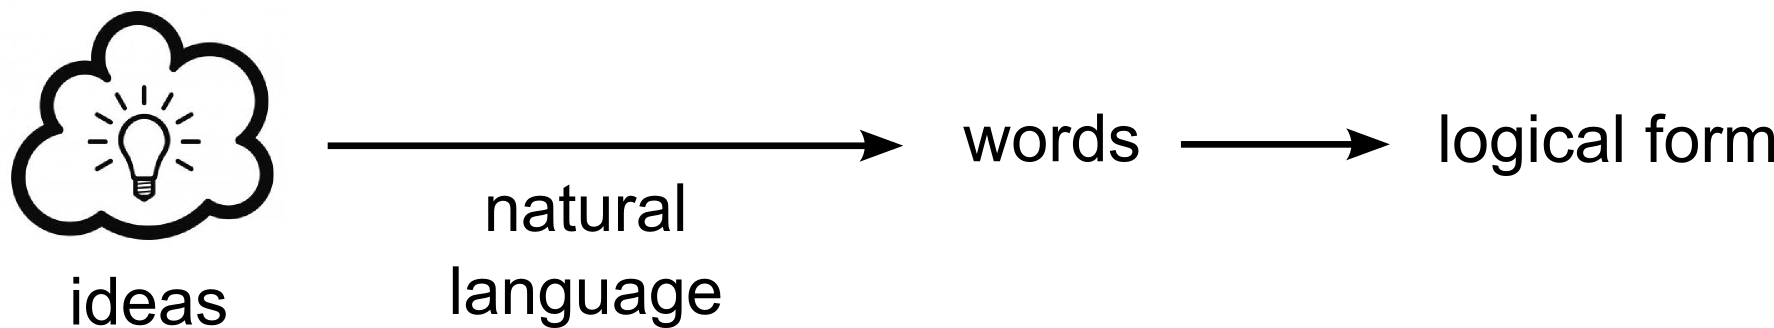
\includegraphics[scale=0.5]{ideas-vs-logical-form.png}
\end{equation}
but is it valid (or profitable) to assume that our mental representations are \textit{isomorphic} to such logical structures?  Or drastically different?

Humans are good at designing symbolic structures, but we don't know how to design \textit{neural} representations which are more or less opaque to us.
Perhaps we could use a neural network acting recurrently on the state vector to \textbf{induce} an internal representation of mental space.  ``\textit{Induced by what},'' you ask?  By the very structure of the neural network itself.  In other words, forcing a neural network to \textit{approximate} the ideal operator $R^*$.

From an abstract point of view, we require:
\begin{itemize}
\item $R$ be an endomorphism: $X \rightarrow X$
\item $R$ has a learning algorithm: $R \stackrel{A}{\longmapsto} R^*$
\end{itemize}

$R$ would contain all the knowledge of the KB, so we expect it to be ``large'' (eg. having a huge number of parameters).  We also desire $R$ to possess a \textbf{hierarchical} structure because hierarchies are computationally very efficient.  A multi-layer perceptron (MLP) seems to be a good candidate, as it is just a bunch of numbers (weight matrices $W$) interleaved by non-linear activation functions:
\begin{equation}
R(\vect{x}) = \sigmoid(W_1 \sigmoid(W_2 ... \sigmoid(W_L \vect{x} )))
\end{equation}
where $L$ is the number of layers.  MLPs would be our starting point to explore more design options.

In 1991 Siegelmann and Sontag \cite{Siegelmann1991} proved that recurrent neural networks (RNNs) can emulate any Turing machine.  In 1993 James Lo \cite{Lo1993} proved that RNNs can universally approximate any non-linear dynamical system.

The idea of $R$ as an operator acting on the state is inspired by the ``consequence operator'' in logic, usually denoted as $\mbox{Cn}$:
\begin{equation}
\mbox{Cn}(\Gamma) = \{ \mbox{ set of propositions that entails from } \Gamma \; \}
\end{equation}
but the function of $R$ can be broader than logical entailment.  We could use $R$ to perform the following functions which are central to LBAI:
\begin{itemize}
\item \textbf{deduction} -- forward- and backward-chaining
\item \textbf{abduction} -- finding explanations
\item \textbf{inductive learning}
\end{itemize}

\begin{tcolorbox}[width=\textwidth,colback={white},title={\centering \textbf{Example 1: } primary-school arithmetic},colbacktitle=white,coltitle=black]

A recurrent neural network is a \textit{much more powerful} learning machine than a feed-forward network, even if they look the same superficially.

\begin{wrapfigure}{l}{2cm}
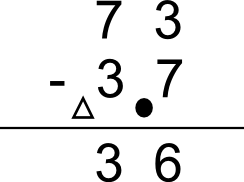
\includegraphics[scale=0.6]{elementary-arithmetic.png}
\end{wrapfigure} 

As an example, consider the way we perform 2-digit subtraction in primary school.  This is done in two steps, and we put a dot on paper to mark ``carry-over''.

The use of the paper is analogous to the ``tape'' in a Turing machine -- the ability to use short-term memory allows us to perform much more complex mental tasks.

We did a simple experiment to train a neural network to perform primary-school subtraction.  The operator is learned easily if we train the two steps \textit{separately}.  The challenge is to find an algorithm that can learn \textbf{multi-step} operations by itself.

\end{tcolorbox}

\begin{tcolorbox}[width=\textwidth,colback={white},title={\centering \textbf{Example 2: } variable binding in predicate logic},colbacktitle=white,coltitle=black]

The following formula in predicate logic defines the ``grandfather'' relation:

\begin{equation}
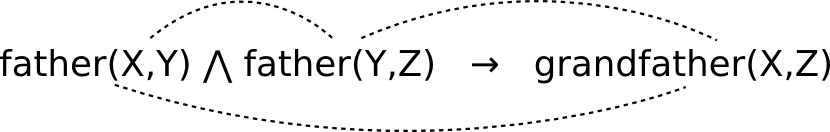
\includegraphics[scale=0.75]{linkage-in-logic-variables.png}
\end{equation}


We did a simple experiment to train a neural network to perform primary-school subtraction.  The operator is learned easily if we train the two steps \textit{separately}.  The challenge is to find an algorithm that can learn \textbf{multi-step} operations by itself.

\end{tcolorbox}  

In LBAI, logic possesses additional structure:
\begin{itemize}
\item \textbf{truth values} (eg. P(rain tomorrow) = 0.7)
\item \textbf{propositional structure} (eg. conjunction: $A \wedge B$) 
\item \textbf{sub-propositional structure} (eg. predication: loves(john, mary) )
\item \textbf{subsumption structure} (eg. $\mbox{dog} \subseteq \mbox{animal}$)
\end{itemize}

These structures can be ``transplanted'' to the vector space $X$ via:
\begin{itemize}
\item \textbf{truth values: } an extra dimension conveying the ``strength'' of states
\item \textbf{propositional structure: } eg. conjunction as vector addition,
\begin{equation}
A \wedge B = \vect{x}_A + \vect{x}_B + ...
\end{equation}
but we have to avoid linear dependencies (``clashing'') such as:
\begin{equation}
\vect{x}_3 = a_1 \vect{x}_1 + a_2 \vect{x}_2
\end{equation}
This would force the vector space dimension to become very high.
\item \textbf{sub-propositional structure: } eg. tensor products as composition of concept atoms:
\begin{equation}
\mbox{loves(john, pete)} = \overrightarrow{john} \otimes \overrightarrow{love} \otimes \overrightarrow{pete}
\end{equation}
\item \textbf{subsumption structure: } eg. define the positive cone $C$ such that
\begin{equation}
\mbox{animal} \supseteq \mbox{dog} \quad \Leftrightarrow \quad \overrightarrow{animal} - \overrightarrow{dog} \in C
\end{equation}
\end{itemize}

But the more logical structure we add to $X$, the more it will resemble logic, and this whole exercise becomes pointless.  Remember our original goal is to try something different from logic, by \textit{relaxing} what defines a logical structure.  So we would selectively add features to $X$.


\section{Unifying RL and RNN}

From the viewpoint of reinforcement learning, we aim to learn the \textbf{policy} function: \par
\begin{equation}
\begin{tikzcd}[]
\mbox{policy : ~~state} \arrow[r, mapsto, "\scalebox{0.8}{action}"] & \mbox{state'}
\end{tikzcd}
\end{equation}
Where $K$ can be regarded as the \textbf{mental state}, and thus an \textbf{action} in RL turns $K$ into $K'$.

In our system, there are 2 pathways that act on $K$, via RNN and RL respectively: \par
\begin{equation}
\begin{tikzcd}[column sep=huge]
& K'_1 \arrow[dd, dashed, no head, "\scalebox{1.3}{$\approx$}"] \\
K \arrow[ur, "\mbox{RL}"] \arrow[dr, "\mbox{RNN}"'] & \\
& K'_2
\end{tikzcd}
\end{equation}
In RL, the action $a$ acts on $K$, whereas in RNN, $R$ acts on $K$.

\textbf{Note}: RNN and RL are learning algorithms, and if they are both applied to the same problem, conflicts will necessarily arise, unless there is a way to combine them.

At state $K$, we estimate the Q-value $Q(K \stackrel{a}{\mapsto} K')$.  The action that would be chosen at state $K$ is $\displaystyle \arg\max_a Q(K \stackrel{a}{\mapsto} K')$.  This could be used to train the RNN via $\displaystyle K \vdash_W ...^n K'$.

RL 在众多状态 $K$ 之间游荡,学习 $Q(K \mapsto K')$。  因为 RL 独有奖励讯息,我们必需用 RL 来教导 RNN 学习,反之不可。  第一个问题是: RL 如何在 $K$ 之间游荡?   游荡是随机的,但也可以借助 RNN 的随机性、或在 RNN 自身的游荡中注入更多随机性、或者根本就是 RL 自己产生的随机性。  接下来的问题是: RNN 如何用 $Q$ 值来诱发学习?

RNN 的 ``$n$-fold'' 学习可以通过以下方式实现: 
\begin{itemize}
\item stochastic forward-backward propagation
\item genetic?
\item 最有趣的是 Hebbian learning,因为它似乎特别适合这情况。  
\end{itemize}

RNN 的本质是什么?  它似乎是一个 recurrent hetero-associative memory。  但其实它还需要将 input 作类似於 Word2vec 的 encoding。  这个 encoding 将「相似」的思维状态 $K$ 归到同类。  利用空间中的相似度,RL 可以用一些连续函数来近似 Q 值(详细情况还有待分析)。

另一个问题是: 虽然用函数的近似可以做到 generalization,但另一个方法是利用状态 $K$ 中的空位作暂时储存。 这两者似乎很不同。  问题似乎在於: 状态转换 $K \mapsto K'$ 是不是对应於逻辑中的\textbf{一条} rule?  答案似乎是 yes。  这个共识是很重要的。  如果用 decision tree,需要的是向量空间中的相似度。

现在的关键是「状态变量」。  因为它可以做到符号逻辑中靠变量的 generalization,这是前所未有的。  这种 generalization 似乎不需要相似度,因为它是符号的!  会不会在向量空间中的状态变量 能够做到之前逻辑变量做不到的动作?  不管怎样,用 RNN 学习这些变量的动作似乎是很难的,因为这些动作似乎不是对\textbf{误差}的梯度下降。  除非这些动作本身也近似於其他动作,但那是怎样的近似?  学习 multi-step logic 其实和以前的 forward / backward chaining 没有分别!  唯一分别是命题的 representation 改变了,它未必像符号的 concatenation。  所以问题仍然是 ``$n$-fold'' 学习法。 

而且注意: RL 的 generalization 根本上不同於 rules 空间中的 generalization。 前者是思维空间 $K$ 中的一般化,后者也可以是 $K$ 空间的一般化,但也可以是依赖「状态变量」的一般化。

一般来说,RL 和 RNN 的行动和学习,是可以互相独立的。  

还有 heterarchical 的分类法。  想用 decision tree 或什么,达到不同网络的\textbf{分工}。  在组织知识这方面,深度网络有没有用?  可以想像,在视觉识别中,在网络的最上层有很多 objects,而它们都可以还原到底层的 features。  网络有更多层,可以识别的事物更抽象。  但现在我们要的不是\textbf{模式识别},而是 mapping。 特别是抽象模式的 mapping。  想要的是: 大量的 rules,将不同的 $K$ 映射到新的 $K'$。

还有一点要澄清的是: 究竟每一个「思元素」在向量空间中是不是\textbf{一点}?  如果有了这个「思元素 = 点」假设,则每次 iteration 应该会删除一个思元素,而用另一个(全新的)思元素取代之。  这样,$K \mapsto K'$ mapping 就有了更确定的结构。  这样的 setup 已经很接近 logic 系统,但其学习算法仍然很有 combinatorial 的 ``feel''。 (因为只有当两个 rules 串连之后,才能达到某个结论,而这个串连有没有中间的 continuous 状态?)  这种串连通常是怎样找到的?  

现在有一转机: 如果「思元素 = 点」,则「状态变量」的形成似乎会很普遍,而我们可以集中研究如何学习 single-step rules。 RL 的 rewards 可以指导学习,但这些「终极 rewards」对学习的细节没有指导作用。  我们似乎可以用「\textbf{时间延迟}」来达到「状态变量」的效果,这个做法无形中增加了使用状态变量的机会。  

现在总结一下仍然有待回答的问题:
\begin{itemize}
\item RL 的 generalization 如何做?
\item iterative thinking map 如何 learn?
\item 
\end{itemize}

Hebbian 的情况是: 有某一 I/O pattern; 我想 strengthen 这 pattern。 

Assuming the learning is correct, $K'_1$ and $K'_2$ should be roughly the same \textemdash~ but this ignored the possibility that one path may take multiple steps to converge with the other path.  \footnote{This situation has been encountered in term rewriting systems (TRS):  If in a TRS any 2 different rewriting paths always converge to the same result, it is said to have the \textbf{Church-Rosser property}.  For example the $\lambda$-calculus invented by Church has this property.} 

Now I stipulate that $R$ be more ``refined'', that is to say, applying $D^n$ times may be equivalent to applying $a$ once:
\begin{equation}
\begin{tikzcd}[column sep=huge]
& K'_1 \arrow[dd, dashed, no head, "\scalebox{1.3}{$\approx$}"] \\
K \arrow[ur, "\scalebox{1.3}{$a$}"] \arrow[dr, "{\scalebox{1.3}{$D^n$}}"'] & \\
& K'_2
\end{tikzcd}
\end{equation}
Using a different notation, $a$ is the \textbf{restriction} or \textbf{section} of $D^n$ at point $K$: $a = D^n|_K$.

Now the question is, do the RNN and RL paths have any \textit{essential} difference?
\begin{itemize}
\item Their internal \textbf{representations} are different:\par
\dashh RNN is a multi-layer neural network\par
\dashh RL's representation is $Q(\mbox{state},\mbox{action})$, usually stored as a \textit{look-up table}, although $Q$ could be approximated by a neural network as well.
\item RL learns through \textbf{rewards}, RNN learns from \textbf{errors}.  Thus RL has broader applicability, because not all questions have ``correct answers'' that could be measured by errors.  In RL we just need to praise Genifer whenever she displays good behavior.
\item The internal cognitive state $K$ exists because of RNN:  it is simply the vector input and output of the RNN.  Without this $K$, RL would be clueless as to what are its internal states.  It can be said that the RNN provides a \textit{machinery} for RL to control.
\end{itemize}

% programming needed:
% RNN: with special back-prop
% RL: approximate Q(K,a), using special NN that can find max also

% 整体来说,RL 可以操控的 actions 包括:
% \begin{enumerate}[\tab (A)]
% \item apply $K \stackrel{D}{\mapsto} K'$ \par
% 但注意: $K$ 是认知状态,$R$ 是对 $K$ 进行「合乎逻辑的推论」。 所以,无论发生什么事,我们都会将 $R$ 作用在 $K$ 上几次。 换句话说,$R$ 是\ds{必然}进行的动作,或者可以看成是在\ds{背景}下进行的运作,所以不需要用 RL 学习。 %RL 的用处是学习如何在很多 actions 之间选择最好的一个,所以 $R$ 不是 RL 需要学习的 action,它只是。

% \item 改写认知状态 $K \mapsto K'$ \par
% RL 的 actions (A) 是
% 在思考过程中改变 $K$ 的值。 例如我们得到一个局部结论,这个局部结论的状态不是最终答案,但也比什么都没有的效用更高。 改写 $K$ 的方法可以是: 例如 将 $K \mbox{ += } \delta K$,或者 「if $K \in$ 某 region,then $K \mbox{ += } \delta K $」。

% \item 学习: change $R$ \par

From the perspective of reinforcement learning, we could reward some results of multi-step inference: \par
\begin{equation}
\begin{tikzcd}[row sep=tiny]
x_0 \arrow[r, mapsto, "a"] & x_\vdash \quad \updownarrow \bigstar
\end{tikzcd}
\end{equation}
$\updownarrow \bigstar$ means ``to give positive or negative rewards''.  We want to learn $a$ which is the action to be taken at state $K$.  The learning algorithm is based on the famous \textbf{Bellman optimality condition} (see next section).

Perhaps we should use RL to \textit{guide} the learning in RNN, as RNN is more fine-grained....

To combine the 2 learning approaches, we could use the technique of \textbf{interleaving}: for each step apply RL once, apply RNN $n$ times.

% 但 $R$ 本身是 RNN,它还可以透过 back-prop 进行学习,两者似乎是不同的。  Back-prop 是透过 $\frac{\partial}{\partial D}(\mbox{error})$ 的梯度来学习。

The learning in RNN may also involve \textbf{neurogenesis} (adding new neurons and connections), but I have not considered this aspect yet.

% RNN 的 $R$ 也是将 $K$ 变成 $K'$ 的作用:\par
%\begin{figure}[h]
%\centering
%\begin{tikzcd}[row sep=tiny]
%K \arrow[r, mapsto, "\scalebox{1.3}{$R$}"] & K'
%\end{tikzcd}
%\end{figure}
% $R$ 和 RL 的 actions 是不一样的。

There are 4 learning modes:
\begin{itemize}
\item learning to listen/talk
\item RL-based learning
\item inductive learning
\end{itemize}

\section{Misc points}

\begin{itemize}
\item If sigmoid is replaced by polynomial, universal approximating property may be retained.

\item Banach fixed point theorem does not apply because $R$ in general need not be contractive.  Question is whether $R$ necessarily converges to fixed points and the answer is no.

\item If reasoning operator $R$ is continuous, the flow of the dynamical system is governed by an autonomous differential equation.  Poincare-Bendixson only applies to dynamical systems on the plane, and is irrelevant to systems whose phase space has dimension $\geq 3$, or to discrete dynamical systems.

\item Time can be discrete or continuous.

\item Goal is to find minimizer of error (ie, to approximate a function given some input-output data points).  The (finite) set of local minima can be solved via setting $\frac{\partial R}{\partial W} = 0$.  The number of local minima can be calculated as: ?  McClelland paper.

\item If operator is discontinuous, what advantages can be gained?
\end{itemize}

What I want to do now is to determine if $R$ implemented as a deep network is sufficient to model human-level reasoning.

One principle seems to be that logical conclusions must not proliferate indefinitely.  But we are not sure what kind of structural constraints this would impose on the vector space.  Or whether we should impose such constraints manually.

What other properties are desired for the implementation of $R$?

\section{Architecture}

First, cartoon version:
\begin{equation}
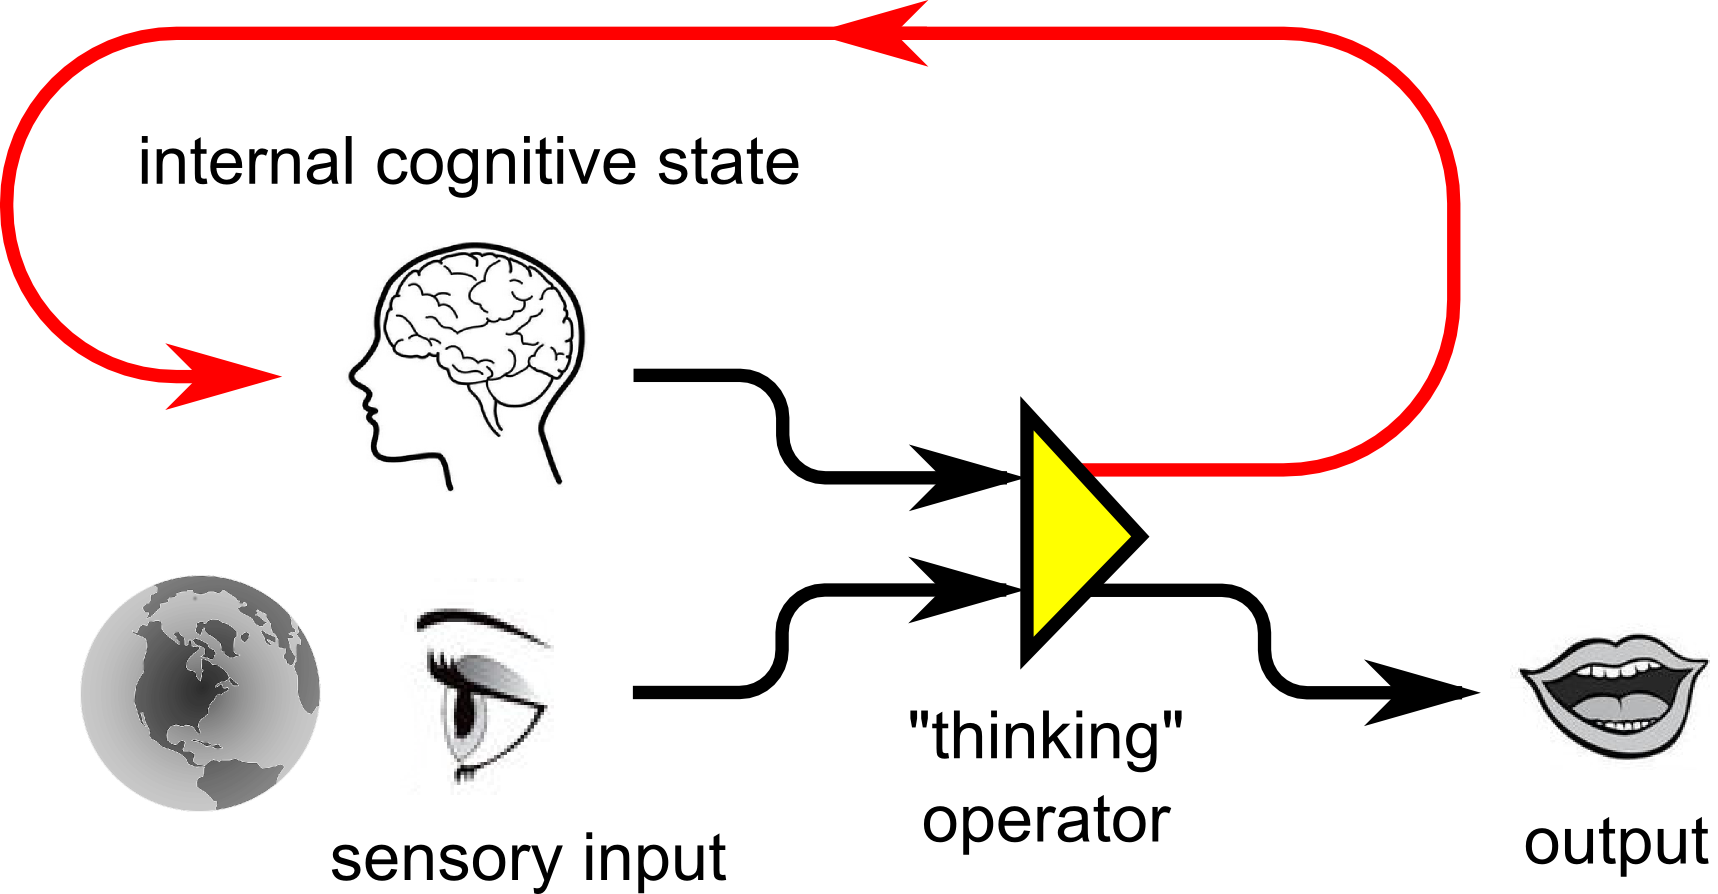
\includegraphics[scale=0.5]{architecture-cartoon.png}
\end{equation}

\begin{equation}
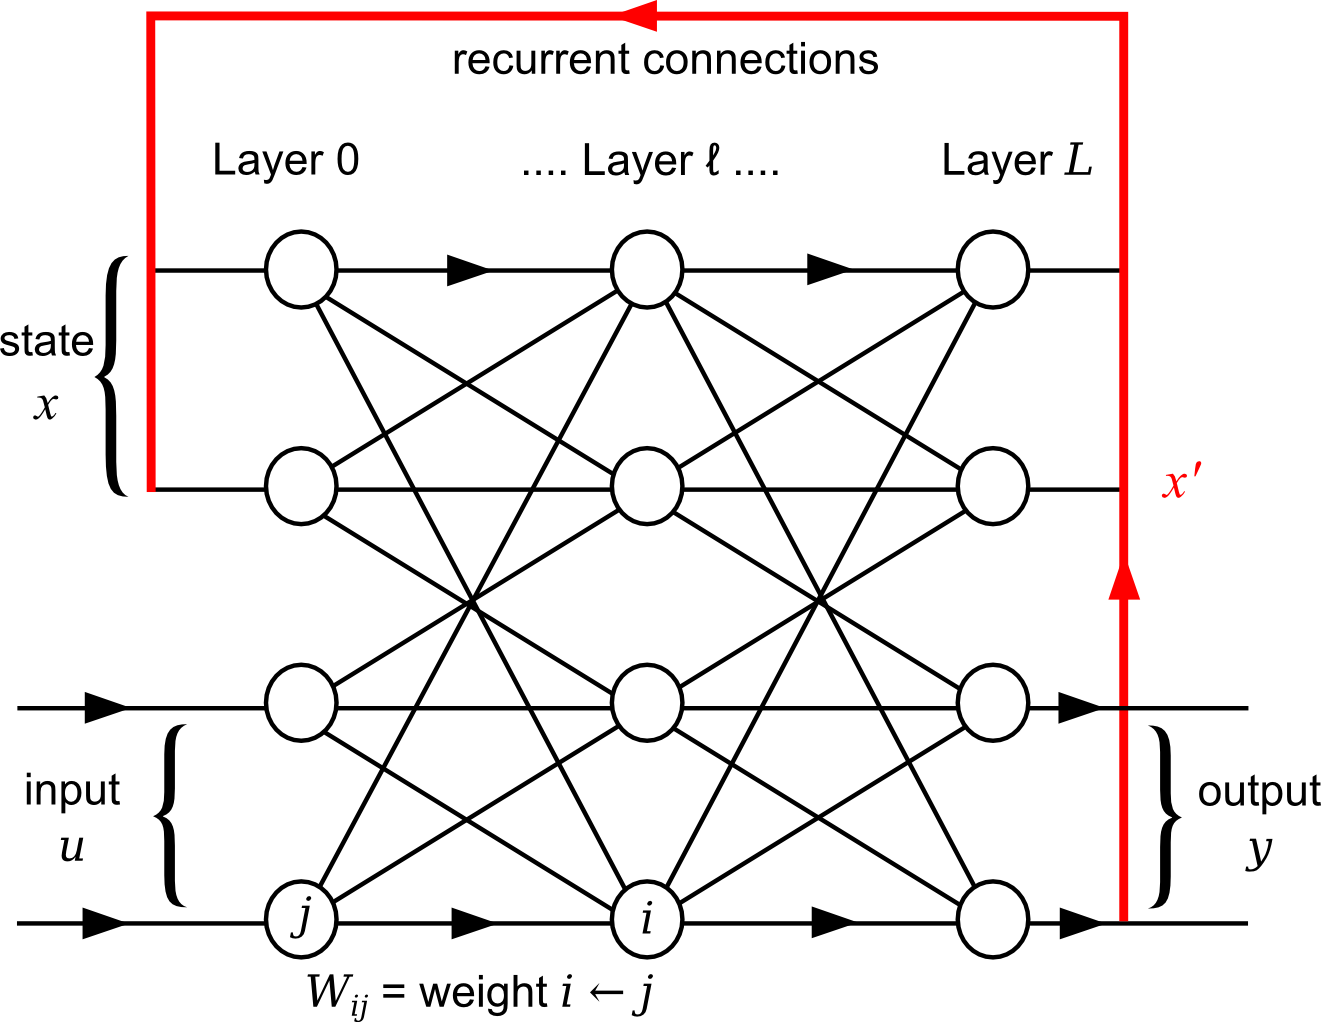
\includegraphics[scale=0.5]{RNN-topology.png}
\end{equation}

TO-DO:  The state space $X$ may be too large and we may need an \textbf{attention mechanism} to select some parts of $X$ for processing by $R$.  This is the notion of \textbf{working memory} in cognitive science.
\begin{equation}
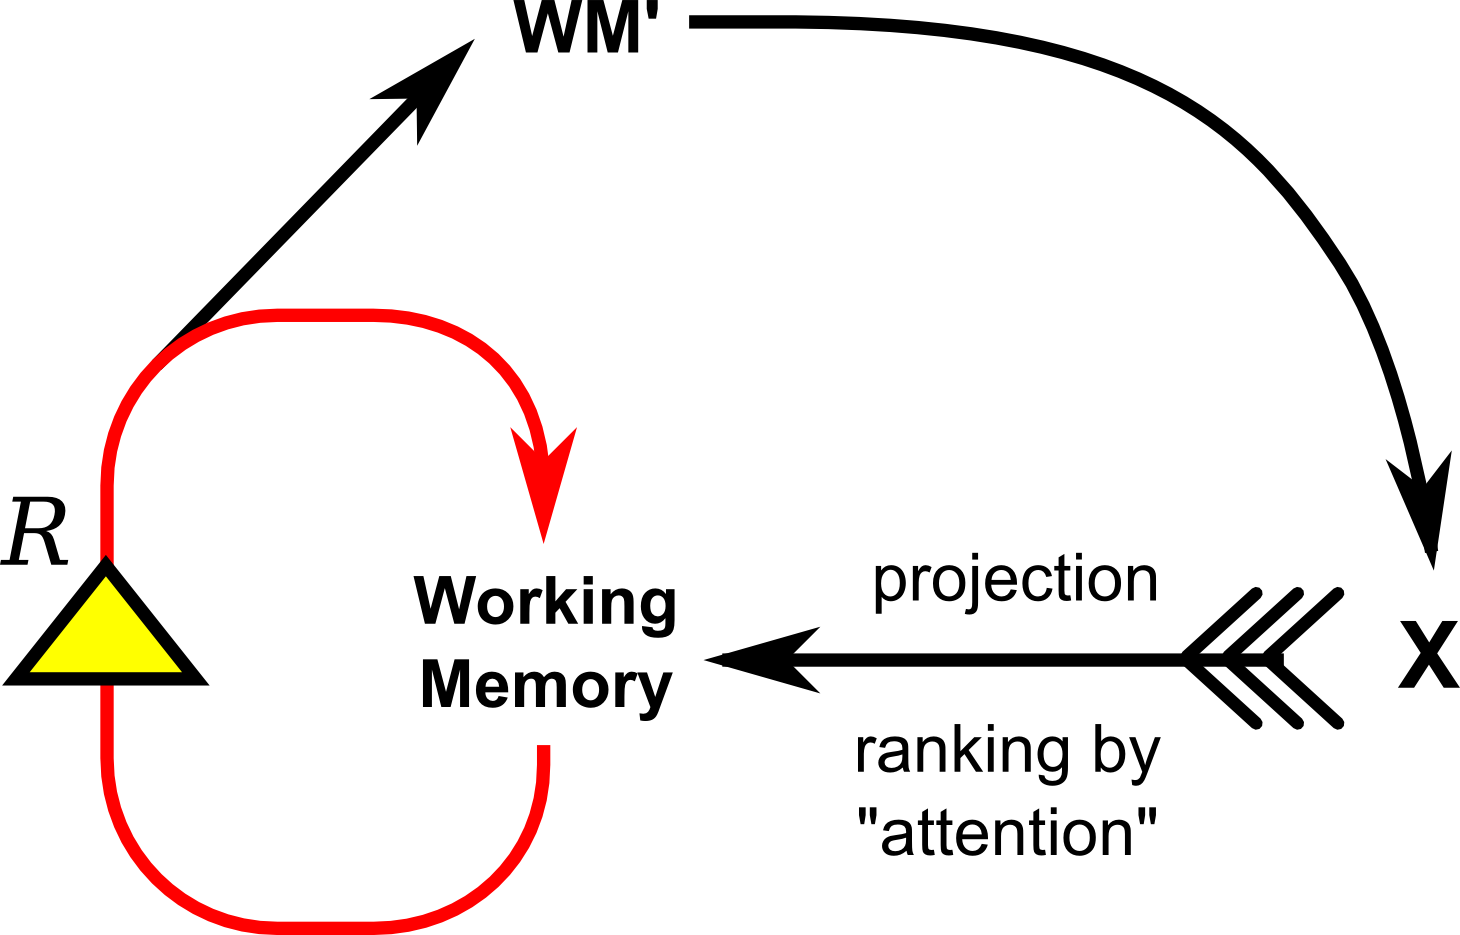
\includegraphics[scale=0.4]{working-memory.png}
\end{equation}

\section{Deep Recurrent Learning}

The learning algorithm for $R$ is central to our system.  $R$ learns to recognize input-output pairs $( \vect{x}_0, \vect{x}^* )$.  What makes it special is that $R$ is allowed to iterate a \textit{flexible} number of times before outputting an answer.  In feed-forward learning we simply learn single-pass recognition, whereas in common recurrent learning we train against a \textit{fixed} time sequence.  Here, the time delay between input and output is allowed to stretch arbitrarily.

Suppose the recurrent network $R$ iterates $n$ times:
\begin{equation}
\vect{x}_{t+1} = \overbrace{R \circ R \circ ...}^{n} (\vect{x})
\end{equation}

As $n \rightarrow \infty$, we get the continuous-time version (a differential equation):
\begin{equation}
\frac{d\vect{x}(t)}{dt} = \mathfrak{R}(\vect{x}(t))
\end{equation}

We could run the network $R$ for a long enough time $T$ such that it is highly likely to reach an equilibrium point.  Then:
\begin{equation}
\vect{x}_{T} = \int_0^T \mathfrak{R}(\vect{x}(t)) dt
\end{equation}
and the error:
\begin{equation}
% \mathscr{E} = \vect{x}^* - \vect{x}_{T}
\boxed{误差} = \vect{x}^* - \vect{x}_{T}
\end{equation}
where $\vect{x}^*$ is the target value which is independent of time.
\begin{eqnarray}
\frac{\partial\mathscr{E}}{\partial\vect{W}} &=& - \frac{\partial}{\partial\vect{W}} \int_0^T \mathfrak{R}(\vect{x}(t)) dt \nonumber \\
&=& - \frac{\partial}{\partial\vect{W}} \int_0^T \sigmoid(W_1 \sigmoid(W_2 ... \sigmoid(W_L \vect{x}(t))) dt
\end{eqnarray}

When there are many layers or if the recurrence is too long, back-prop learning becomes ineffective due to the \textbf{vanishing gradient} problem.  One solution is to use the \textbf{rectifier} activation function:
\begin{equation}
\rectifier (x) = 
\begin{cases}
x, & \mbox{if } x \geq 0 \\
0, & \mbox{otherwise}
\end{cases}
\end{equation}
Since its derivative is piecewise constant, it does not suffer from the vanishing gradient problem.

\subsection{Forward-backward Algorithm}

This is inspired by forward- and backward-chaining in LBAI.  We propagate the state vector from both the initial state $\vect{x}_0$ as well as the final state $\vect{x}^*$.  This bi-directional propagation is added with noise and repeated many times, thus implementing a \textbf{stochastic local search}:

\begin{equation}
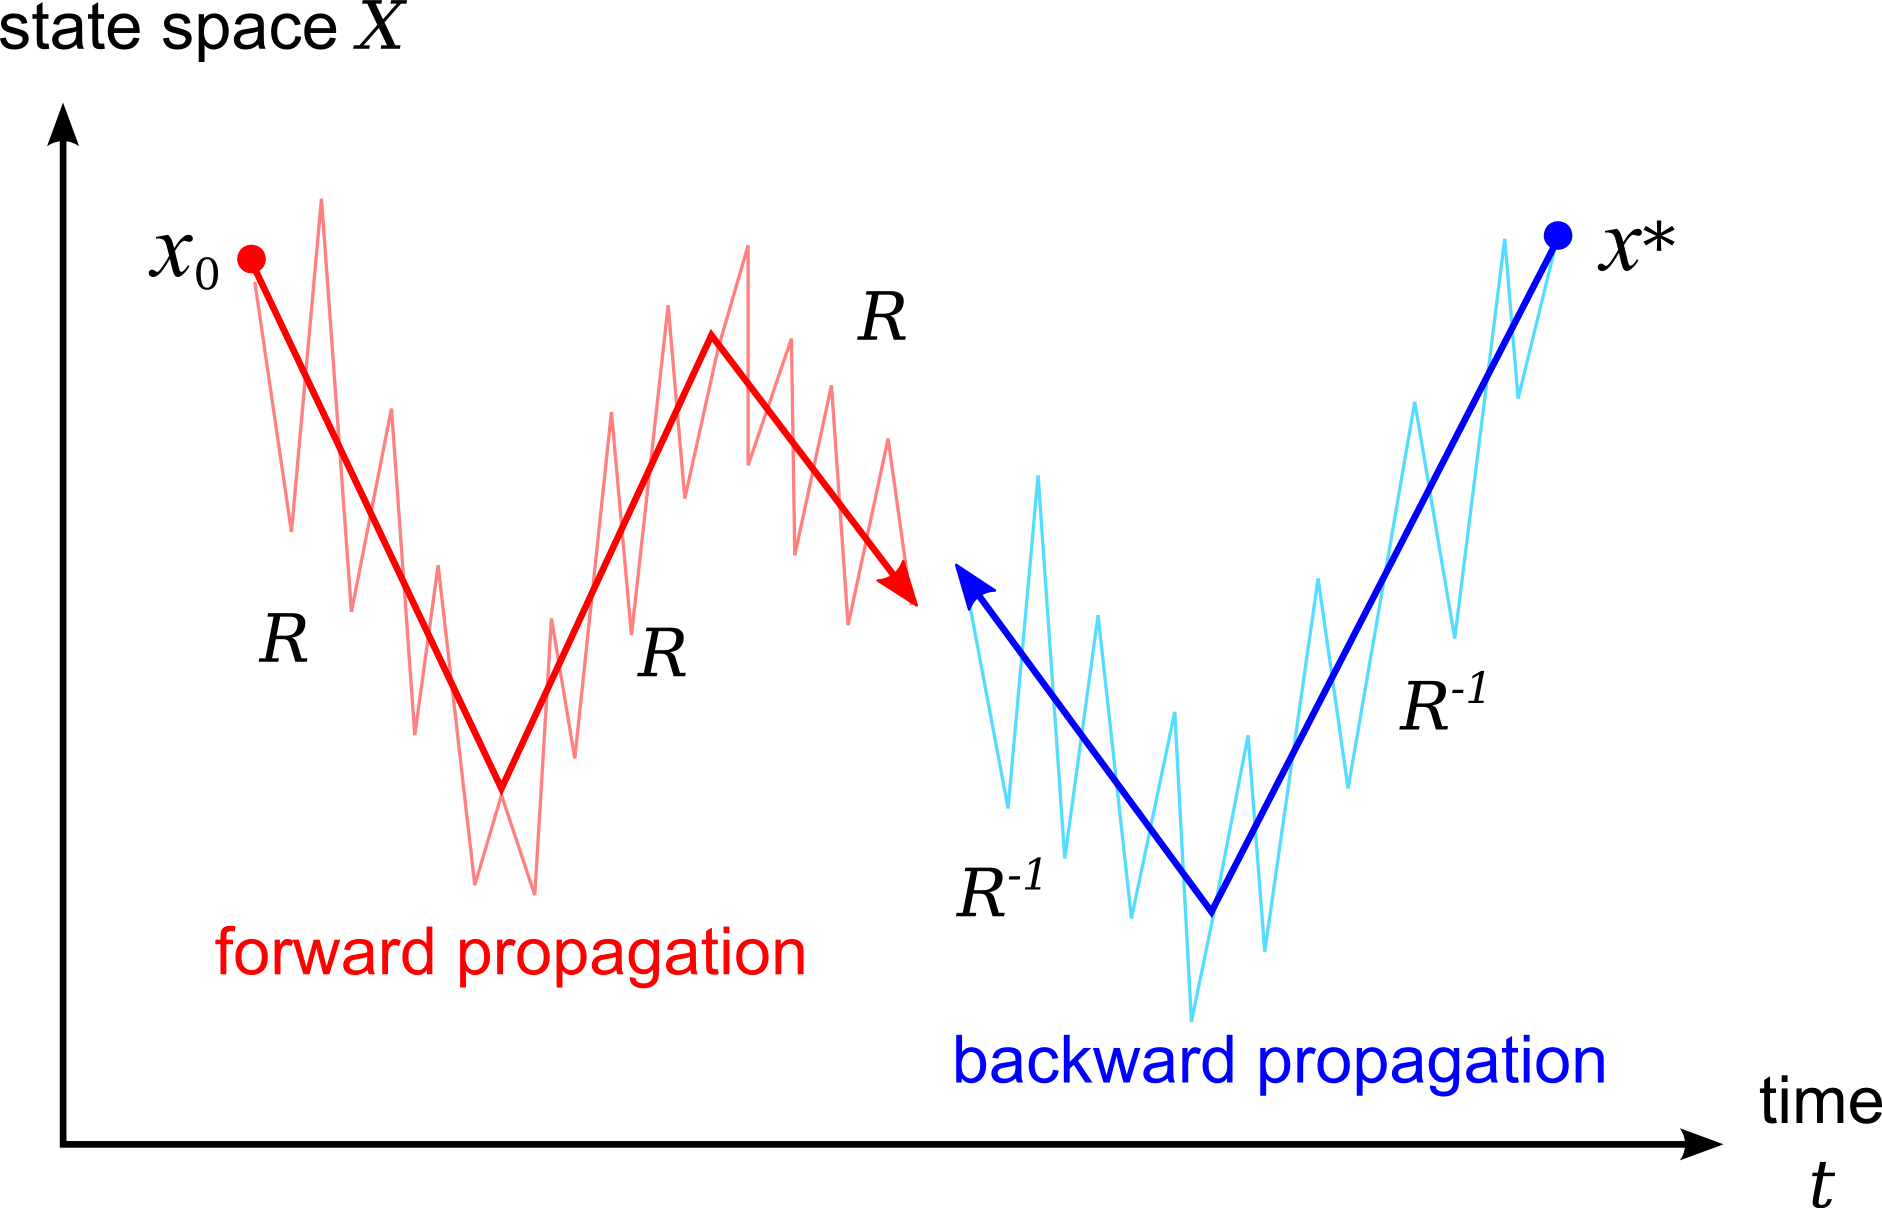
\includegraphics[scale=0.6]{forward-backward-algorithm.png}
\end{equation}

When the forward and backward states get close enough, a successful path is found, and we record the gap and the noises along the path, and use them to train $R$ so that this new path would be recognized.

% One key question is how to deal with "don't care" bits?  One answer is that their errors are zero.  But then this is the same as the error for "correct" weights, which seems not well.  There's got to be a way to alter weights when the answer is correct...

% For \# Iteration = 0, output is immediately known, so potentially the training can be done.  But how to convey that all these alterations of weights are \textbf{optional}?

\section*{Acknowledgements}

\footnotesize{In a forum discussion with Ben Goertzel dated 25 June 2014 on the AGI mailing-list: (artificial-general-intelligence @googlegroups.com), YKY asked: Why bother with neural networks, which typically require many neurons to encode data, when logic-based AI can represent a proposition with just a few symbols?  Ben's insight is that neural networks are capable of learning its own representations, and their learning algorithms are relatively fast.  We have been working on "neo-classical" logic-based AI for a long time, and begin to realize that inductive learning in logic (based on combinatorial search in a symbolic space) is perhaps \textit{the bottleneck} in the entire logic-based paradigm.  So we try to look for alternatives that might enable learning to be faster, though we would still emphasize that logic-based AI remains a viable approach to AGI. %, provided that the right search heuristics be found (most probably in the form of \textbf{hierarchical organization} of the learning space).
}

\bibliographystyle{plain} % or number or aaai ...
\bibliography{AGI-book}

\end{document}
